\section{Absicherung}

\subsection{Architektur und Design}
Die SDA Topologie sollte nach den gleichen Designprinzipien und Best Practices aufgebaut werden, welche auch ein Campus-Design verfolgt. Das folgende Beispiel zeigt die physikalische Topologie eines dreistufigen Campus-Designs, bei dem alle Komponenten innerhalb der Fabric redundant sind.

\begin{figure}[H]
	\centering
	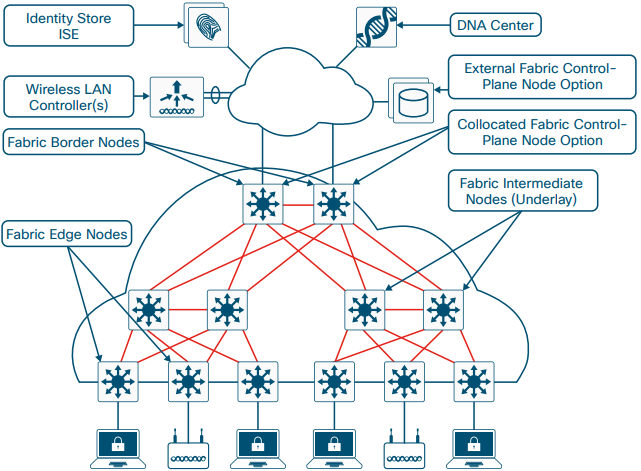
\includegraphics[width=0.8\linewidth]{img/Absicherung/SDA-Architektur}
	\caption{SDA Topologie \cite{sda-designguide-sept2018} }
	\label{fig:SDA Topologie}
\end{figure}

Analog zu dieser wurde die von der Studienarbeit übernommene Architektur (siehe Abbildung \ref{fig:Architektur Studienarbeit}: Architektur Studienarbeit) weiter angepasst und wenn möglich die Komponenten inklusive Verkabelung redundant ausgelegt. Ebenfalls zu beachten sind die Deployment Capabilities, welche als Border und Control Plane Node die Catalyst 3850 empfehlen. Darum werden in der Architektur die Catalyst 9300 als Intermediate oder Edge Nodes eingesetzt. Extended Nodes wie der C3560CX werden zudem nur unterstützt, wenn sie an einem C9300 Edge angeschlossen sind. \\
Diese neu erarbeitete Architektur (siehe Abbildung \ref{fig:Architektur Bachelorarbeit}: Architektur Bachelorarbeit) verfügt über eine grosse Fabric \textit{Deutschschweiz}, welche die zwei Sites \textit{Dübendorf} und \textit{Emmen} beinhaltet. Der Standort \textit{Dübendorf} beinhaltet ein Gebäude der \textit{Luftwaffe}. Der Standort \textit{Emmen} beinhaltet den \textit{Flugplatz}, sowie eine \textit{Kaserne}.


\begin{figure}[H]
	\centering
	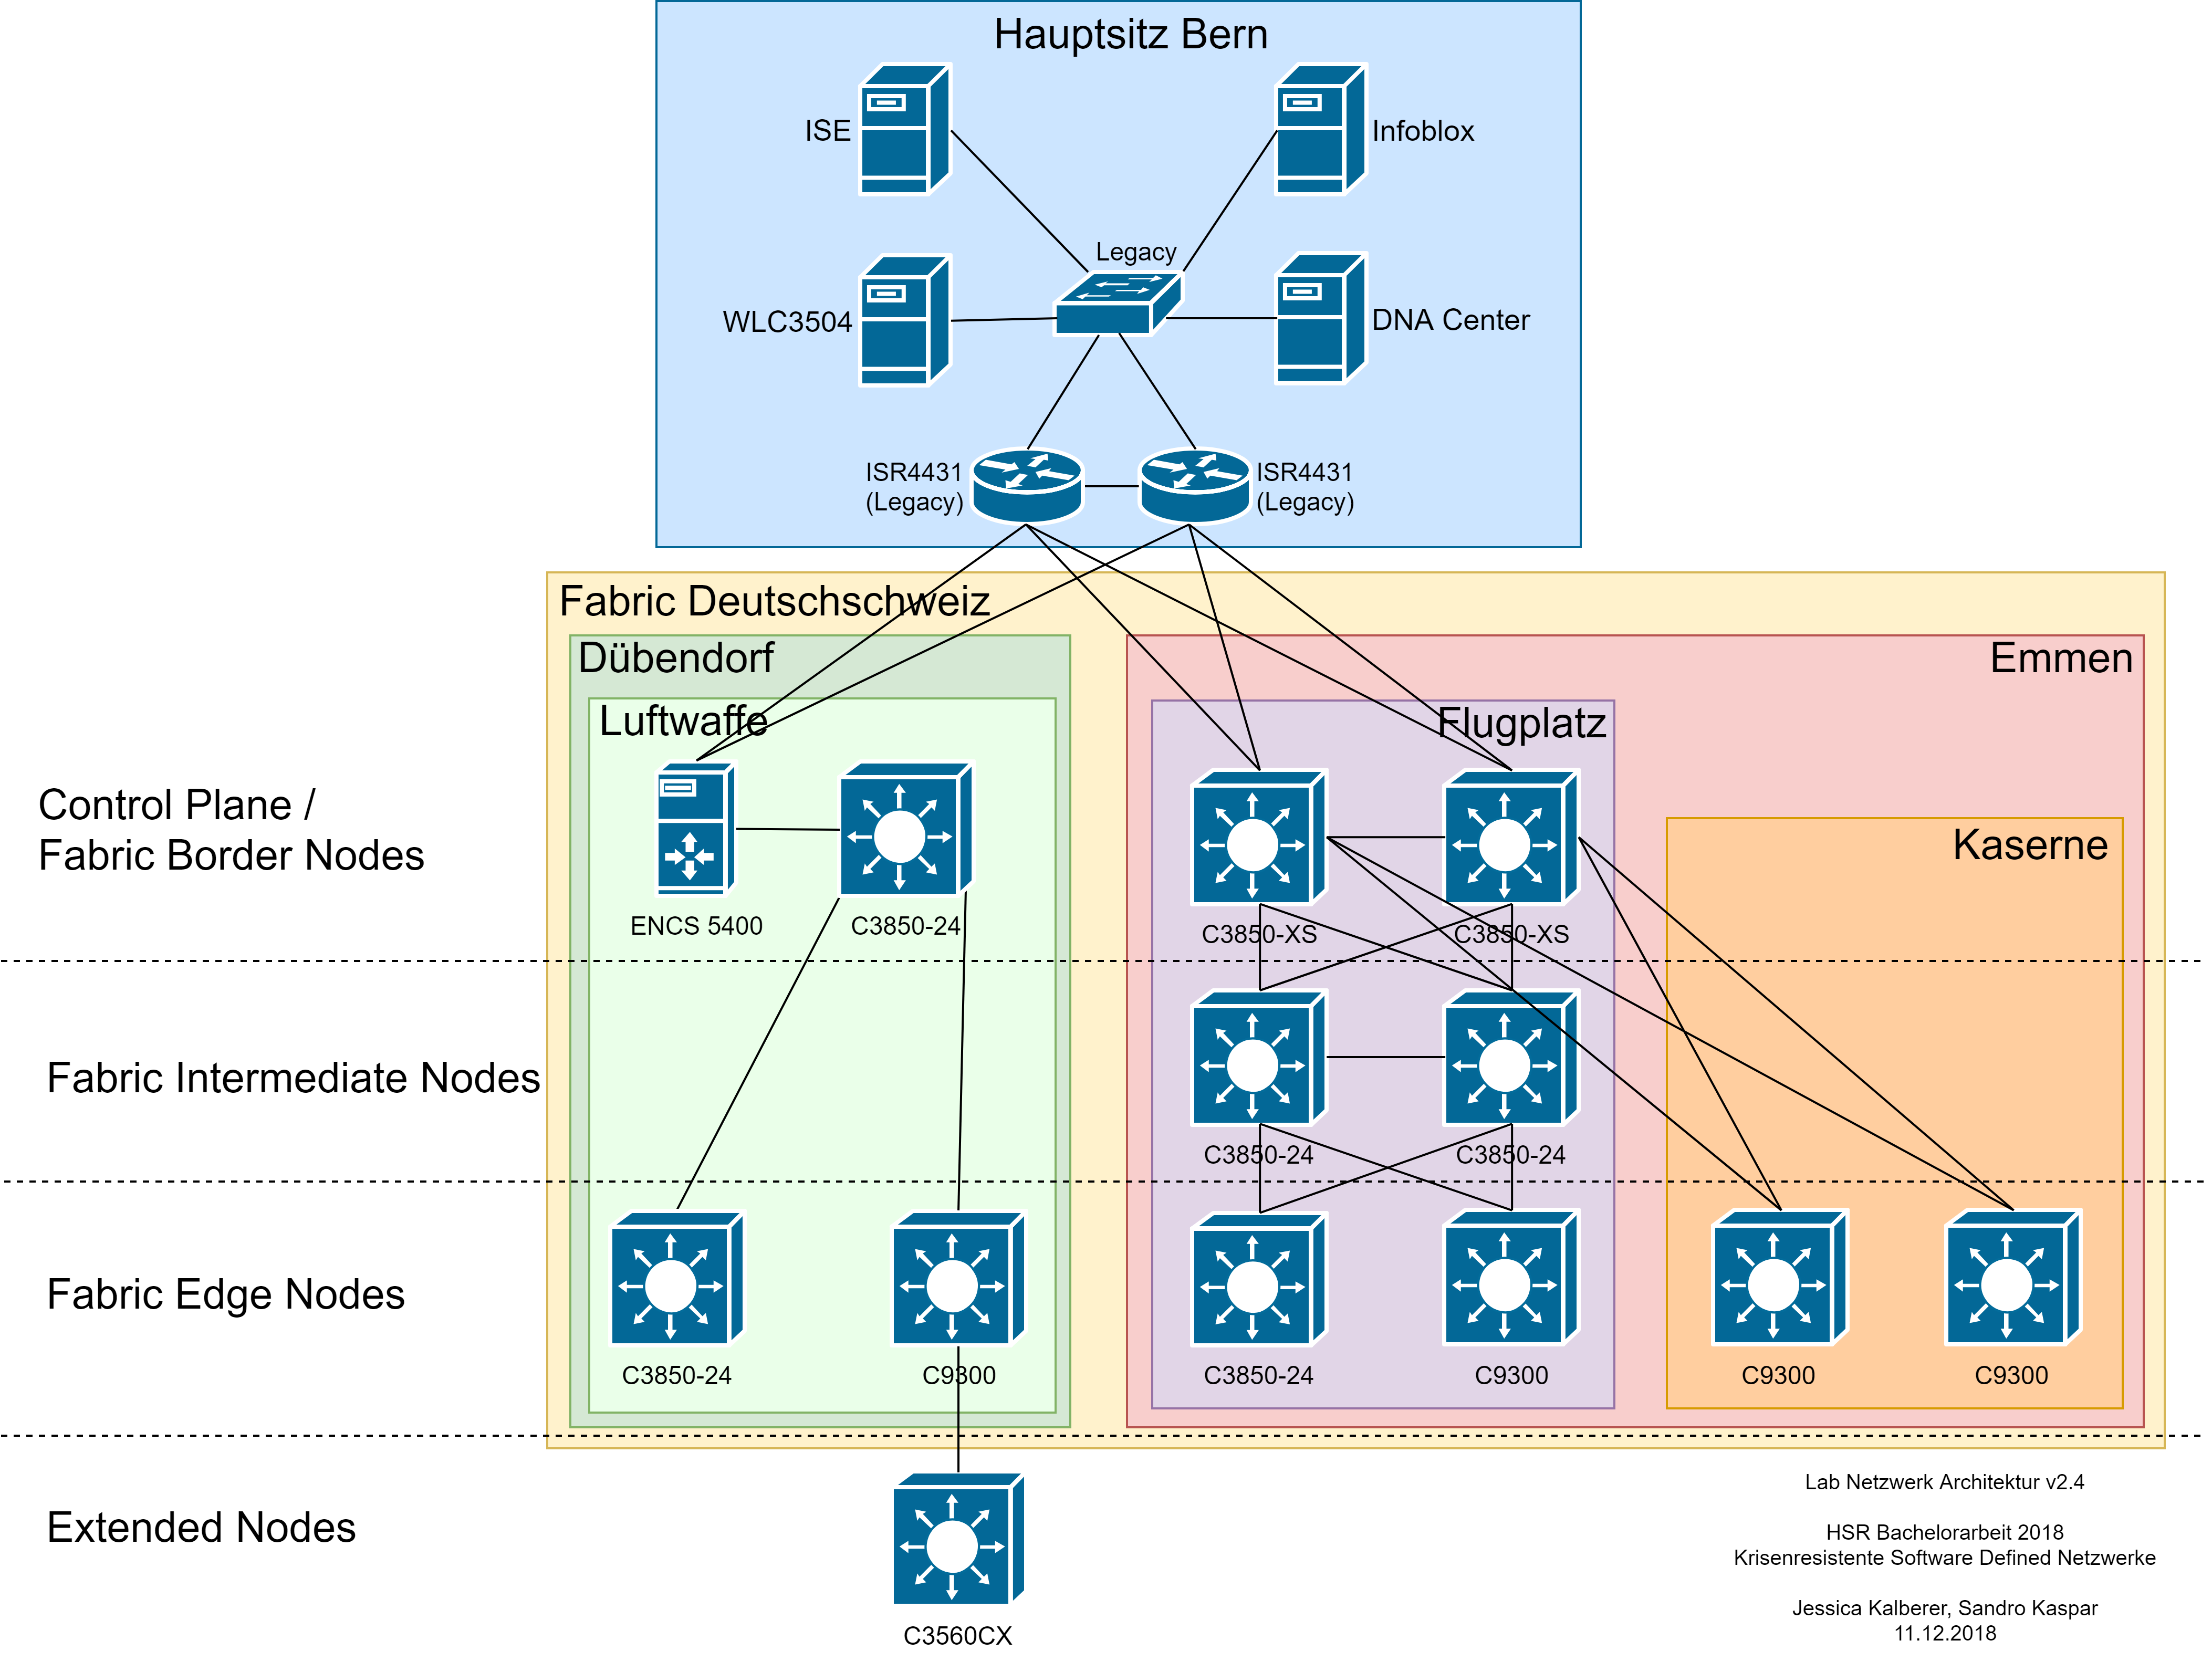
\includegraphics[width=1\linewidth]{img/Architecture/LabNetworkArchitecture-11-12}
	\caption{Architektur Bachelorarbeit}
	\label{fig:Architektur Bachelorarbeit}
\end{figure}




\subsubsection{Extended Nodes}
In einer SDA-Lösung werden Netzwerkgeräte wie der Catalyst 3560CX als Extended Nodes bezeichnet. Der  Extended Node wird verwendet, um nachgeschaltete Nicht-Fabric Layer2 Netzwerkgeräte an die SDA-Fabric anzuschliessen und somit die Fabric zu erweitern.
Der erweiterte Knoten ist ein Gerät wie zum Beispiel ein kleiner Switch (Compact Switch, Industrial Ethernet Switch oder Building Automation Switch), der eine Verbindung zum Fabric Edge Knoten herstellt
über Layer 2. Geräte, die mit dem Extended Node verbunden sind, verwenden den Fabric Edge Nodes für die Kommunikation mit externen Subnetzen.  \\

Um einen Extended Node zu implementieren, sind zur Zeit noch einige manuelle Schritte notwendig.

\paragraph{IP Adress Pool} Damit der Extended Node implementiert werden kann, ist ein IP Adress Pool an der dafür vorgesehenen Site notwendig. Im DNA Center unter \textit{Design $\rightarrow$ Network Settings $\rightarrow$ IP Address Pools} kann mit \textit{Reserve IP Pool} ein neuer IP Pool erstellt werden. Als Type muss unbedingt \textit{LAN} ausgewählt werden.

\begin{figure}[H]
	\centering
	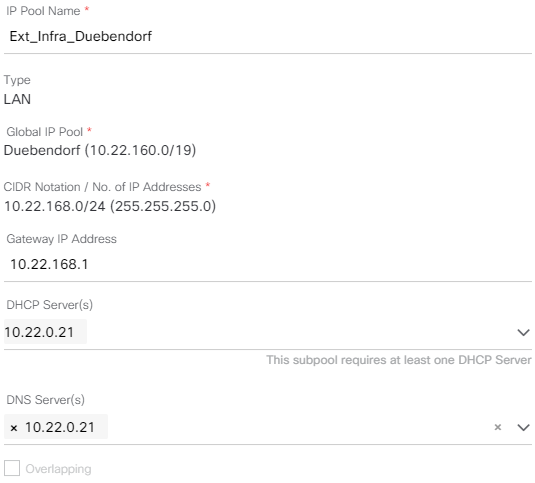
\includegraphics[width=0.6\linewidth]{img/Absicherung/ExtendedNode1}
	\caption{Reserve IP Adress Pool}
	\label{fig:Reserve IP Adress Pool}
\end{figure}

\paragraph{Host Onboarding für Extended Nodes} Als nächstes muss der IP Pool dem dazugehörigen VN zugeordnet werden, damit Extended Nodes am Edge Node erkannt werden. Unter \textit{Provision $\rightarrow$ Fabric} die gewünsche Fabric Domain auswählen. Anschliessend zu der Site navigieren, in welcher sich der Extended Node befinden soll und dort \textit{Host Onboarding} auswählen. Unter \textit{Virtual Networks} das \textit{Infra\_VN} auswählen und den vorher erstellten IP Adress Pool als Extended Pool Type zuweisen. 

\begin{figure}[H]
	\centering
	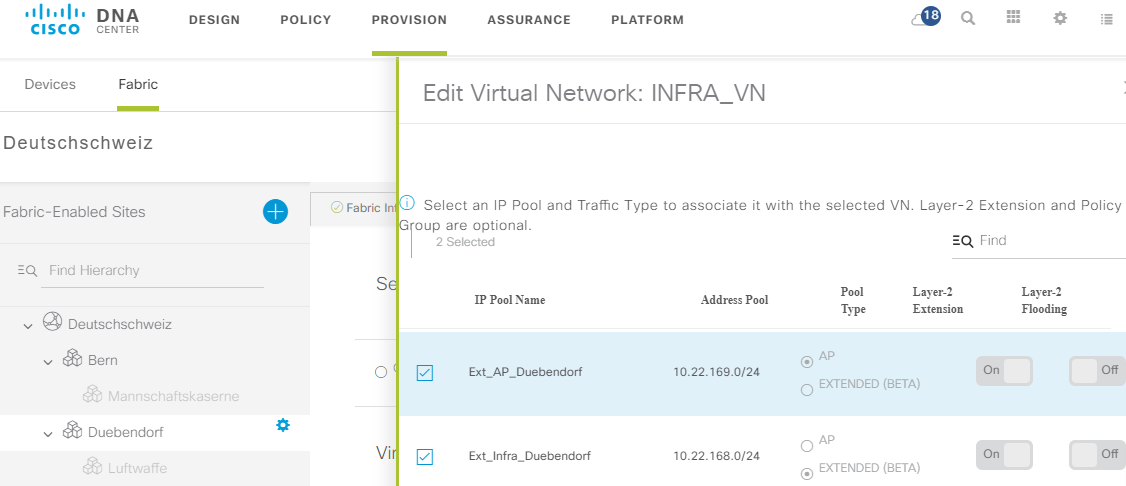
\includegraphics[width=1\linewidth]{img/Absicherung/ExtendedNode2}
	\caption{Virtual Network IP Pool zuweisen}
	\label{fig:Virtual Network IP Pool zuweisen}
\end{figure}

Wichtig ist das dem INFRA\_VN schon ein IP Pool mit dem Pool Type AP zugewiesen ist. Ansonsten muss noch ein IP Pool für dies erstellt und vorher dem Extended dem Infra\_VN zugewiesen werden.

\paragraph{Port Assignment}
Unter \textit{Provision $\rightarrow$ Fabric} die gewünsche Fabric wählen und zur Site navigieren. Nun kann unter \textit{Host Onboarding $\rightarrow$ Select Port Assignment} der Edge Node, an dem der Extended Node angeschlossen wird, ausgewählt werden. Das Interface auswählen und mit \textit{Assign} dem Interface einen Device Type mit dazugehörigem IP Pool zuweisen.

\begin{figure}[H]
	\centering
	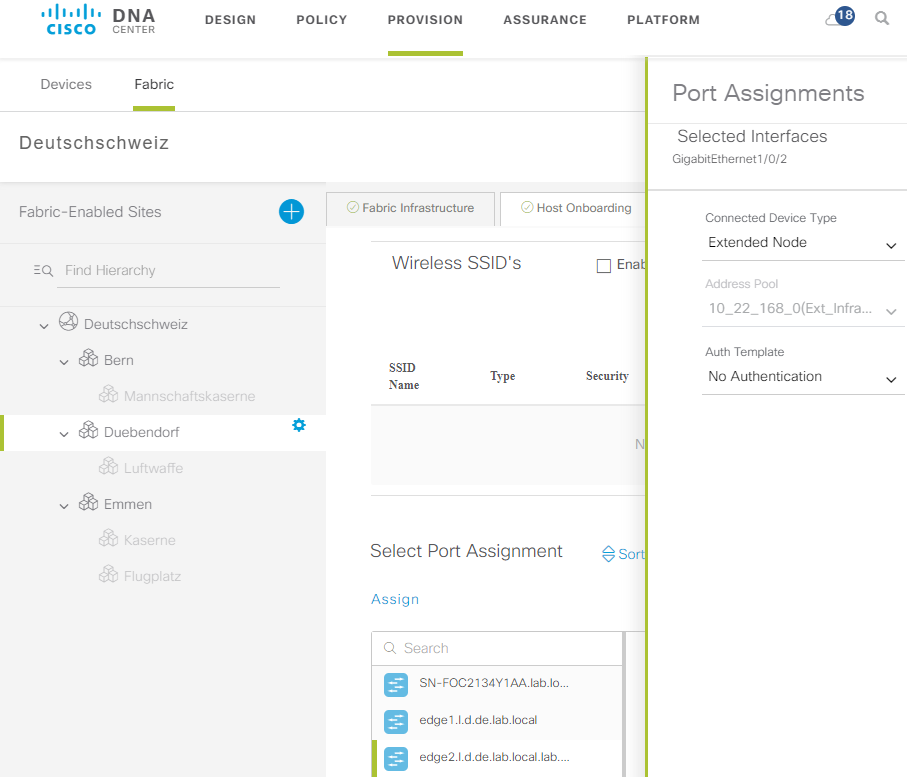
\includegraphics[width=1\linewidth]{img/Absicherung/ExtendedNode3}
	\caption{Port Assignment}
	\label{fig:Port Assignment}
\end{figure}

\paragraph{DHCP Options}
Damit der Extended Node beim booten nun erfolgreich mittels PnP dem DNA Center hinzugefügt wird, müssen dem IP Pool noch DHCP Options angegeben werden. Dafür im Infoblox \textit{Data Management $\rightarrow$ DHCP $\rightarrow$ Networks $\rightarrow$ Networks} den IP Pool auswählen und mit \textit{Edit} editieren. Hier unter \textit{IPv4 DHCP Options $\rightarrow$ Custom DHCP Options} folgende Option hinzufügen:
\begin{itemize}
	\item Option 43 (vendor-encapsulated-option): 5A1D;B2;K4;I[\textit{IP des DNA Center}];J80
\end{itemize}

\paragraph{Extended Node}
Am einfachsten ist es, wenn auf dem Extended Node die Konfiguration gelöscht und er neugestartet wird. Nun sollte der mit dem Fabric Edge Node verbundene Extended Node automatisch von einem Macro erkannt werden, welches auf dem Edge Node ausgeführt wird. Das Macro erkennt den Extended Node und startet den PnP Prozess. Nach Abschluss des Discovery Prozesses wird der neue Extended Node in der Fabric Site Topologie und natürlich auch im Provision Inventory erscheinen. Das Provision Inventory ist unter \textit{Provision $\rightarrow$ Devices $\rightarrow$ Inventory} zu erreichen. Die Site Topologie kann unter \textit{Provision $\rightarrow$ Devices $\rightarrow$ gewünschte Fabric $\rightarrow$ gewünschte Site} angezeigt werden, wie unten im Bild ersichtlich, wird der Extended Node in der Topologie mit \textit{EX} gekennzeichnet.

\begin{figure}[H]
	\centering
	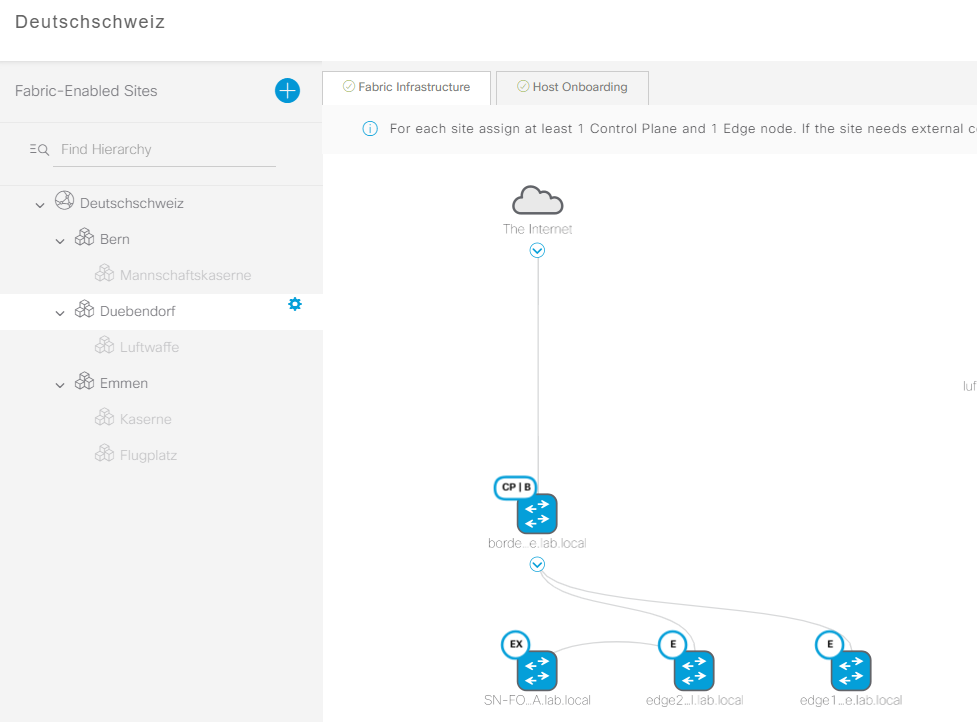
\includegraphics[width=1\linewidth]{img/Absicherung/ExtendedNode4}
	\caption{Fabric Infrastructure}
	\label{fig:Fabric Infrastructure}
\end{figure}



\subsection{ENCS 5400}

Um mit möglichst kleinem Hardwareeinsatz eine maximale Autonomie der Aussenstandorte zu ermöglichen, wird pro Aussenstelle ein oder mehrere ENCS 5400 eingesetzt. 
Dabei handelt es sich um eine Virtualisierungsplattform basierend auf KVM. Des Weiteren beinhaltet die Appliance einen Switch. 
Auf diesem System können virtuelle Router, Firewalls, WLCs und mittels Third Party Images viele weitere Dienste betrieben werden. Für spezifische Anwendungen können eigene Images erstellt werden, wodurch die Plattform enorm vielseitig einsetzbar ist.

\begin{figure}[H]
	\centering
	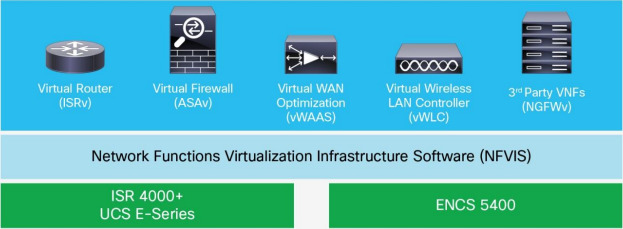
\includegraphics[width=0.8\linewidth]{img/Absicherung/ENCS_Architecture.png}
	\caption{ENCS Architecture \cite{enterprise-network-functions-virtualization-faq} }
	\label{fig:ENCS Architecture}
\end{figure}

\subsubsection{Image erstellen}

In einem ersten Schritt muss ein Disk Image für den gewünschten Service vorliegen. In unserem Fall wurde diese via Virtualbox erstellt, sodass alle nötigen Pakete bereits installiert werden konnten. Da das Image im Format qcow2 vorliegen muss, wird das vdi Image entsprechend konvertiert.

\begin{lstlisting}[language=bash]
qemu-img convert -f vdi -O qcow2 Ubuntu18.04_Branch.vdi \
Ubuntu18.04_Branch.qcow2
\end{lstlisting}

\paragraph{Image Packaging}

Damit das Image verwendet werden kann, muss ein Package erstellt werden. Dabei handelt es sich um ein Archiv, bestehend aus dem Disk Image, sowie einem XML File, in welchem Metadaten, wie die Hardwareanforderungen und die verschiedenen Profile definiert sind.
Das Package kann manuell oder mittels NFVIS Web Interface erstellt werden.

Im Web-Interface wird dies unter \textit{VM Life Cycle $\rightarrow$ Image Repository $\rightarrow$ Image Packaging} erstellt.

\begin{figure}[H]
	\centering
	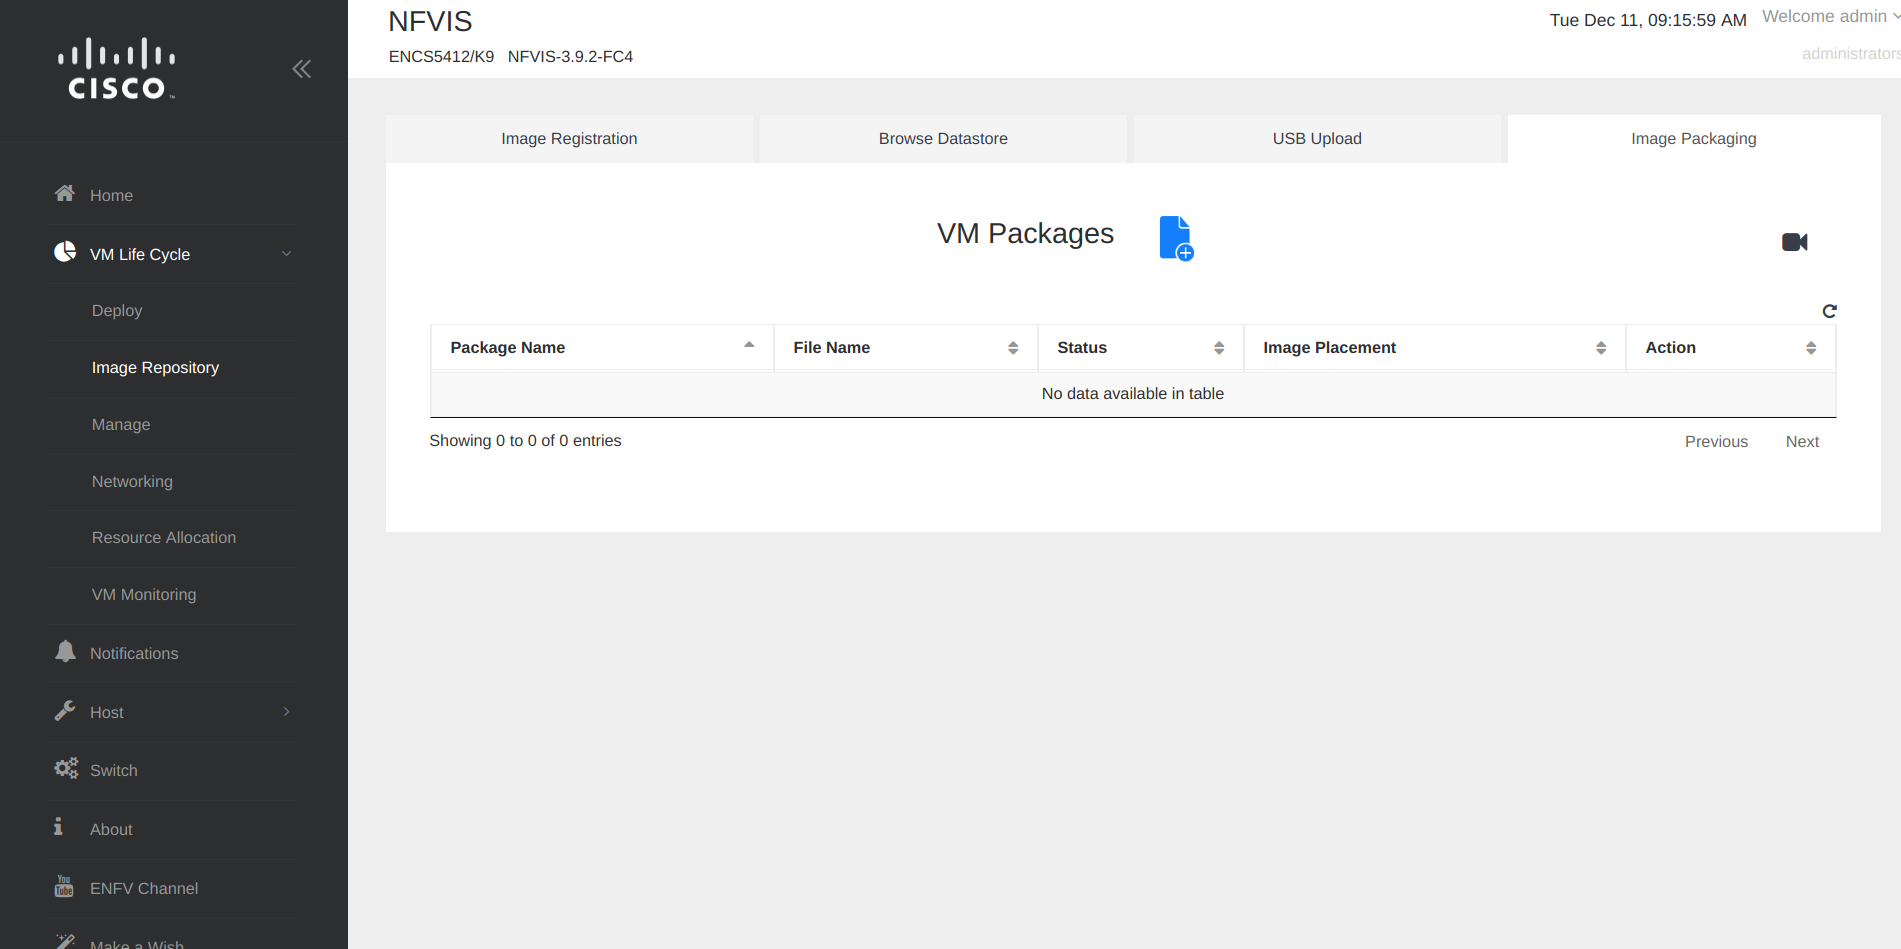
\includegraphics[width=0.8\linewidth]{img/Absicherung/ENCS-Image-Packaging.png}
	\caption{ENCS Image Packaging}
	\label{fig:ENCS Image Packaging}
\end{figure}

\paragraph{Image Konfiguration}

Anschliessend werden die Metadaten für das Image definiert. Diese sind schlussendlich im XML File zu finden.

\begin{figure}[H]
	\centering
	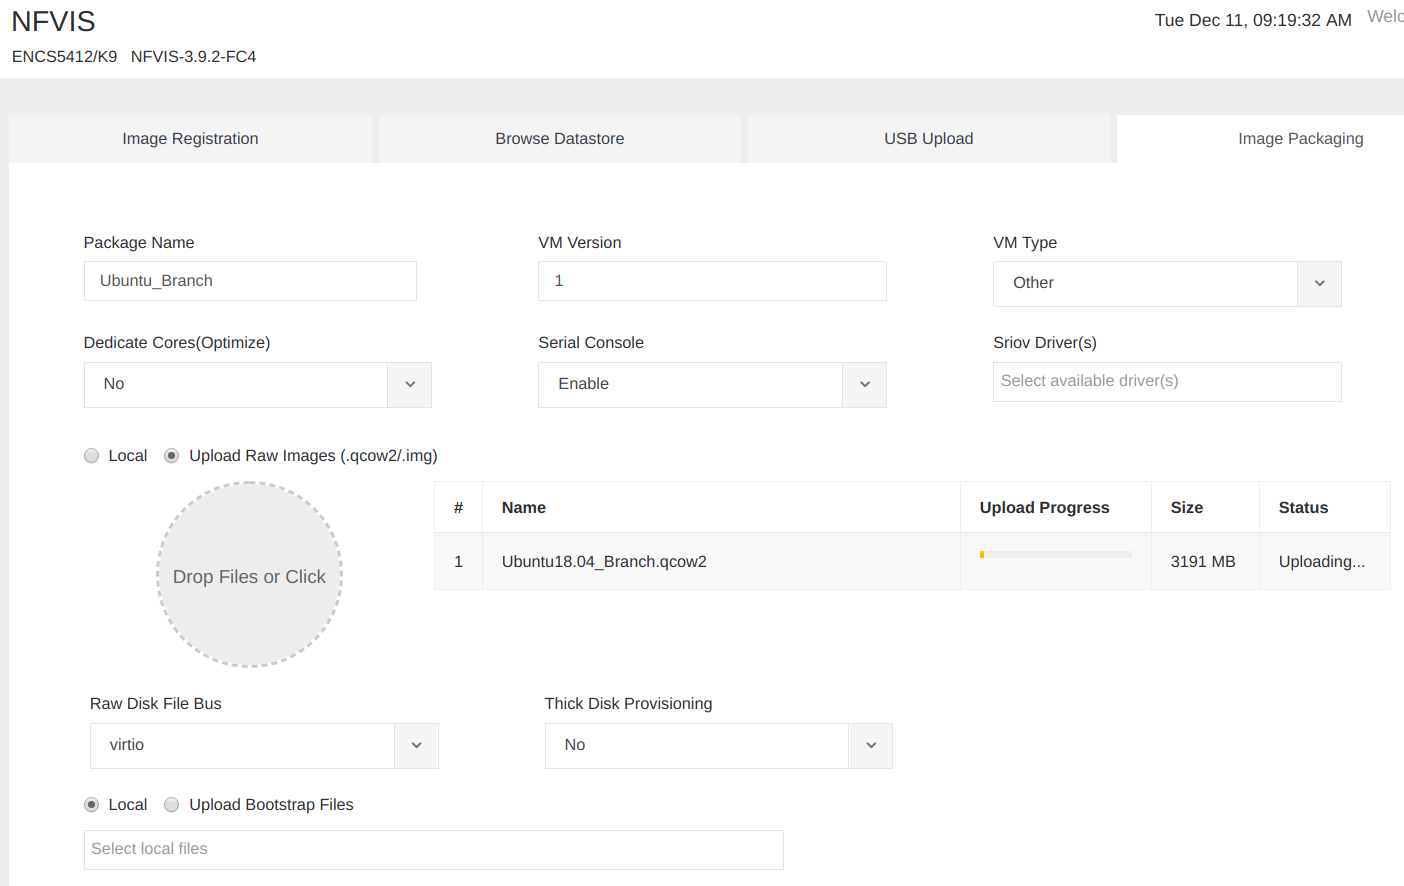
\includegraphics[width=0.8\linewidth]{img/Absicherung/ENCS-Image-Creation.png}
	\caption{ENCS Image Konfiguration}
	\label{fig:ENCS Image Konfiguration}
\end{figure}

Des Weiteren werden die verschiedenen Profile definiert. Diese können später beim Deployment ausgewählt weden, sodass für verschiedene Grössen eines Branches ein passendes Profil ausgewählt werden kann.

\begin{figure}[H]
	\centering
	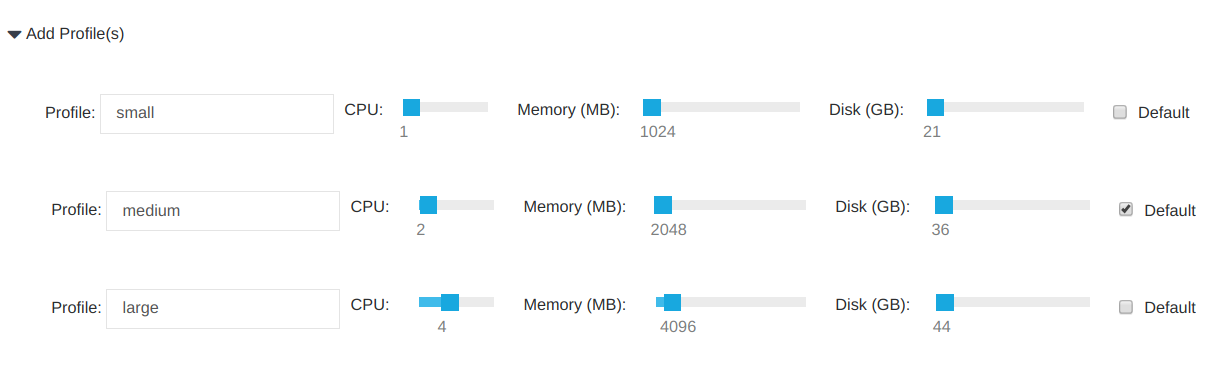
\includegraphics[width=0.8\linewidth]{img/Absicherung/ENCS-Image-Profile.png}
	\caption{ENCS Image Profile}
	\label{fig:ENCS Image Profile}
\end{figure}

\paragraph{Image Deployment}

Das Deployment des Images soll via DNA Center funktionieren. Aus diesem Grund muss das zuvor erstellte Archiv heruntergeladen und anschliessend ins DNA Center importiert werden. \textit{Design $\rightarrow$ Image Repository $\rightarrow$ Virtual $\rightarrow$ Import}

\begin{figure}[H]
	\centering
	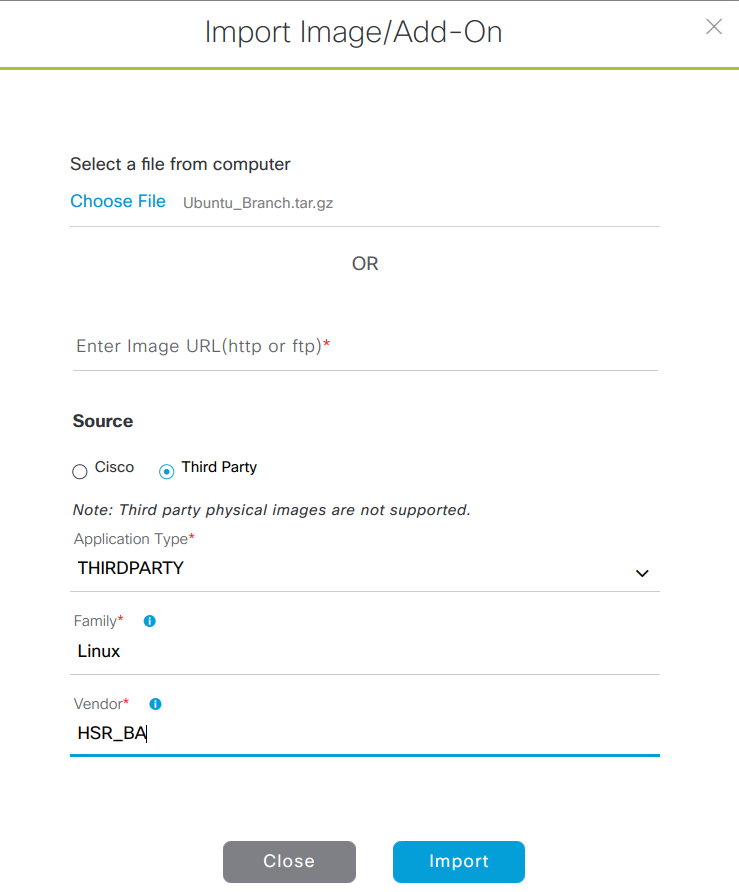
\includegraphics[width=0.8\linewidth]{img/Absicherung/DNA-Center-Image-Import.png}
	\caption{DNA Center Image Import}
	\label{fig:DNA Center Image Import}
\end{figure}





\subsection{DNA Center}
Das DNA Center unterstützt eine Clusterkonfiguration mit einem oder drei Hosts. Im Optimalfall sollte das DNA Center in einem Cluster mit drei Nodes installiert werden. Der Cluster bietet sowohl Software als auch Hardware mit hoher Verfügbarkeit. Das DNA Center bietet einen Mechanismus zum Verteilen der Verarbeitung und Datenbankreplikation auf mehrere Hosts. Durch das Clustering werden Ressourcen und Funktionen gemeinsam genutzt und es werden hohe Verfügbarkeit und Skalierbarkeit ermöglicht. \\

Die folgende Abbildung zeigt die empfohlenen Verbindungen für einen DNA Center Cluster mit drei Knoten. 
\begin{figure}[H]
	\centering
	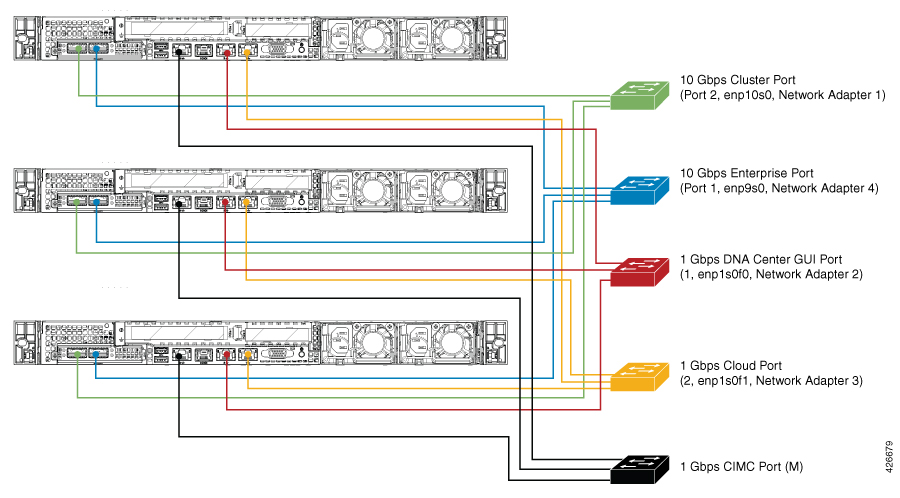
\includegraphics[width=0.8\linewidth]{img/Absicherung/DNAC-Cluster}
	\caption{DNA Center Cluster \cite{dnac-cluster} }
	\label{fig:DNA Center Cluster}
\end{figure}
Alle bis auf eine der Verbindungen für jeden Node im drei Nodes Cluster sind die gleichen wie für den einzelnen Node und verwenden dieselben Ports. Die Ausnahme ist der Cluster-Port (Port 2, enp10so, Network Adapter 1), der erforderlich ist, damit jeder Node im Cluster mit den anderen kommunizieren kann. \\

Für Clusterbereitstellungen mit mehreren Nodes müssen sich alle Cluster Nodes im selben Netzwerk und am selben Standort befinden. Die Appliance unterstützt keine Verteilung von Knoten über mehrere Netzwerke oder Standorte. Diese Limitierung der Bereitstellung, sowie auch die maximale Anzahl der unterstützen Nodes wird sich hoffentlich in Zukunft noch ändern.

Wenn ein Node innerhalb einer Multi-Host-Cluster-Konfiguration ausfällt, beträgt die Zeit für die Wiederherstellung des Clusters in der Regel 20 Minuten. Fällt in einem Multi-Host Cluster mit drei Nodes aus irgendeinem Grund ein einzelner Host aus und es fällt ein zweiter Host aus, so fällt auch der letzte Host sofort aus. Es müssen immer zwei der drei Nodes im Cluster laufen, damit ein funktionsfähiger Cluster noch gewährleistet werden kann.





\subsection{LISP Map Server / Control Plane Node}
Der Control Plane Node ermöglicht LISP und enthält folgende Funktionen:
\begin{itemize}
	\item einen Map Resolver (MR), der Map-Requests von einem ITR entgegennimmt und das EID-zu-RLOC-Mapping mit Hilfe der verteilten Mapping-Datenbank auflöst
	\item einen Map Server (MS), der autoritative EID-zu-RLOC-Mappings von einem ETR lernt und in der Datenbank veröffentlicht
	\item eine Host Tracking Database (HTDB), welche ein zentrales Repository für die EID-zu-Fabric-Edge-Nodes Bindings beinhaltet.
\end{itemize}

Zur Bereitstellung gibt es zwei Varianten. Zum einem kann es einen redundanten globalen MSMR geben, oder es werden pro Fabric ein MSMR implementiert.

\subsubsection{Redundante MS / MR Bereitstellung}

Es wird empfohlen, redundante Standalone MS- und MR-Systeme mit den MS / MR-Funktionen auf demselben Gerät bereitzustellen. Wenn redundante eigenständige MS / MR implementiert werden, müssen sich alle xTRs bei beiden MS registrieren, so dass jeder eine konsistente Sicht auf den registrierten LISP EID-Namespace hat. Für Map-Resolver-Funktionalität ist die Verwendung einer Anycast-IP-Adresse wünschenswert, da dadurch die Mapping-Lookup-Leistung verbessert wird, indem der MR ausgewählt wird, der dem anfordernden ITR am nächsten ist.

\begin{figure}[H]
	\centering
	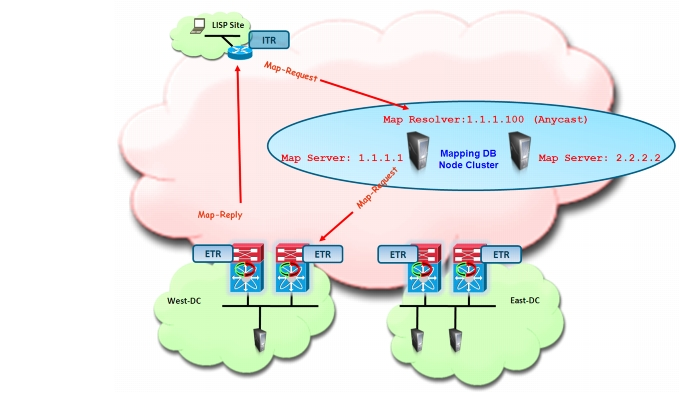
\includegraphics[width=1\linewidth]{img/Absicherung/LISP-Example}
	\caption{Redundante MS / MR Bereitstellung \cite{LISP-mobility} }
	\label{fig:Redundante MS / MR Bereitstellung}
\end{figure}

\subsubsection{Co-Lokalisierung von MS / MR und xTR Funktionalitäten}

Ein weiteres Beispiel ist die Co-Lokalisierung  von MS / MR- und xTR-Funktionalitäten. Das co-lokalisierte Modell ist besonders vorteilhaft, da es die Gesamtzahl verwalteter Geräte reduziert, die zum Ausrollen einer LISP Host Mobility-Lösung erforderlich sind. 

Die erforderliche Konfiguration würde aber in beiden Szenarien identisch bleiben, indem eindeutige IP-Adressen genutzt werden, um die Map-Server und eine Anycast-IP-Adresse für den Map-Resolver zu identifizieren.

\begin{figure}[H]
	\centering
	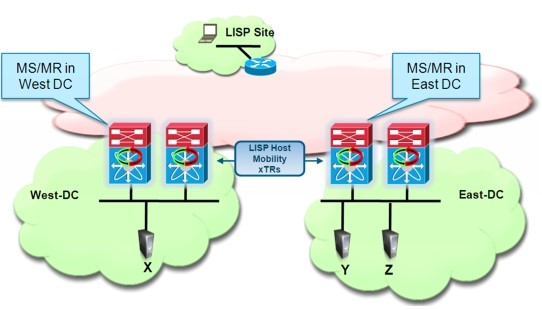
\includegraphics[width=0.8\linewidth]{img/Absicherung/LISP-Example2}
	\caption{Co-Lokalisierung von MS / MR und xTR Funktionalitaeten \cite{LISP-mobility} }
	\label{fig:Co-Lokalisierung von MS / MR und xTR Funktionalitaeten}
\end{figure}

Es kann also ein redundantes eigenständiges MS / MR-Modell bereitgestellt werden, indem dedizierte Systeme zur Durchführung dieser Mapping-Funktionen genutzt werden (siehe Abbildung 2.9) oder alternativ können die MS- und MR-Funktionen gleichzeitig auf dem Netzwerkgerät, welches bereits die xTR-Rolle ausführt, implementiert werden (siehe Abbildung 2.10).

\subsubsection{Anwendung}
Damit bei einem Ausfall eines MSMR nicht alle Fabrics betroffen sind, macht es Sinn pro Fabric einen redundanten MSMR zu implementieren. So können auf einem xTR eine oder mehrere MSMR-Adressen konfiguriert werden.

Abfragen, die ein EID-zu-RLOC-Mapping durchführen, sind datengesteuert. Dieses Verhalten bedeutet, dass ein neuer Datentransfer zwischen LISP-Sites ein Mapping-Lookup erfordert, was dazu führt, dass der Datenversand wird gestoppt, bis ein Mapping durchgeführt wurde. Dies Verhalten ist analog zum DNS-Protokoll und ermöglicht LISP die folgenden Funktionen in einer dezentralen Datenbank mit EID-zu-RLOC-Mappings zu betreiben. 

Die Replikation der gesamten (potenziell umfangreichen) Datenbank ist unnötig, da auf Mappings bei Bedarf zugegriffen wird, genau wie im DNS muss ein Host nicht die komplette Domänendatenbank kennen. Tunnelrouter verwalten den Map-Cache der zuletzt verwendeten Mappings, um die Leistung des Systems zu verbessern.

\paragraph{LISP Client Registration}
Wird ein noch unbekannter neuer Client an die Fabric angeschlossen, sendet der ITR einen Map-Request an einen bekannten MR, wenn es ein EID-zu-RLOC-Mapping benötigt, das noch nicht in seinem lokalen Map-Cache vorhanden ist.

\begin{figure}[H]
	\centering
	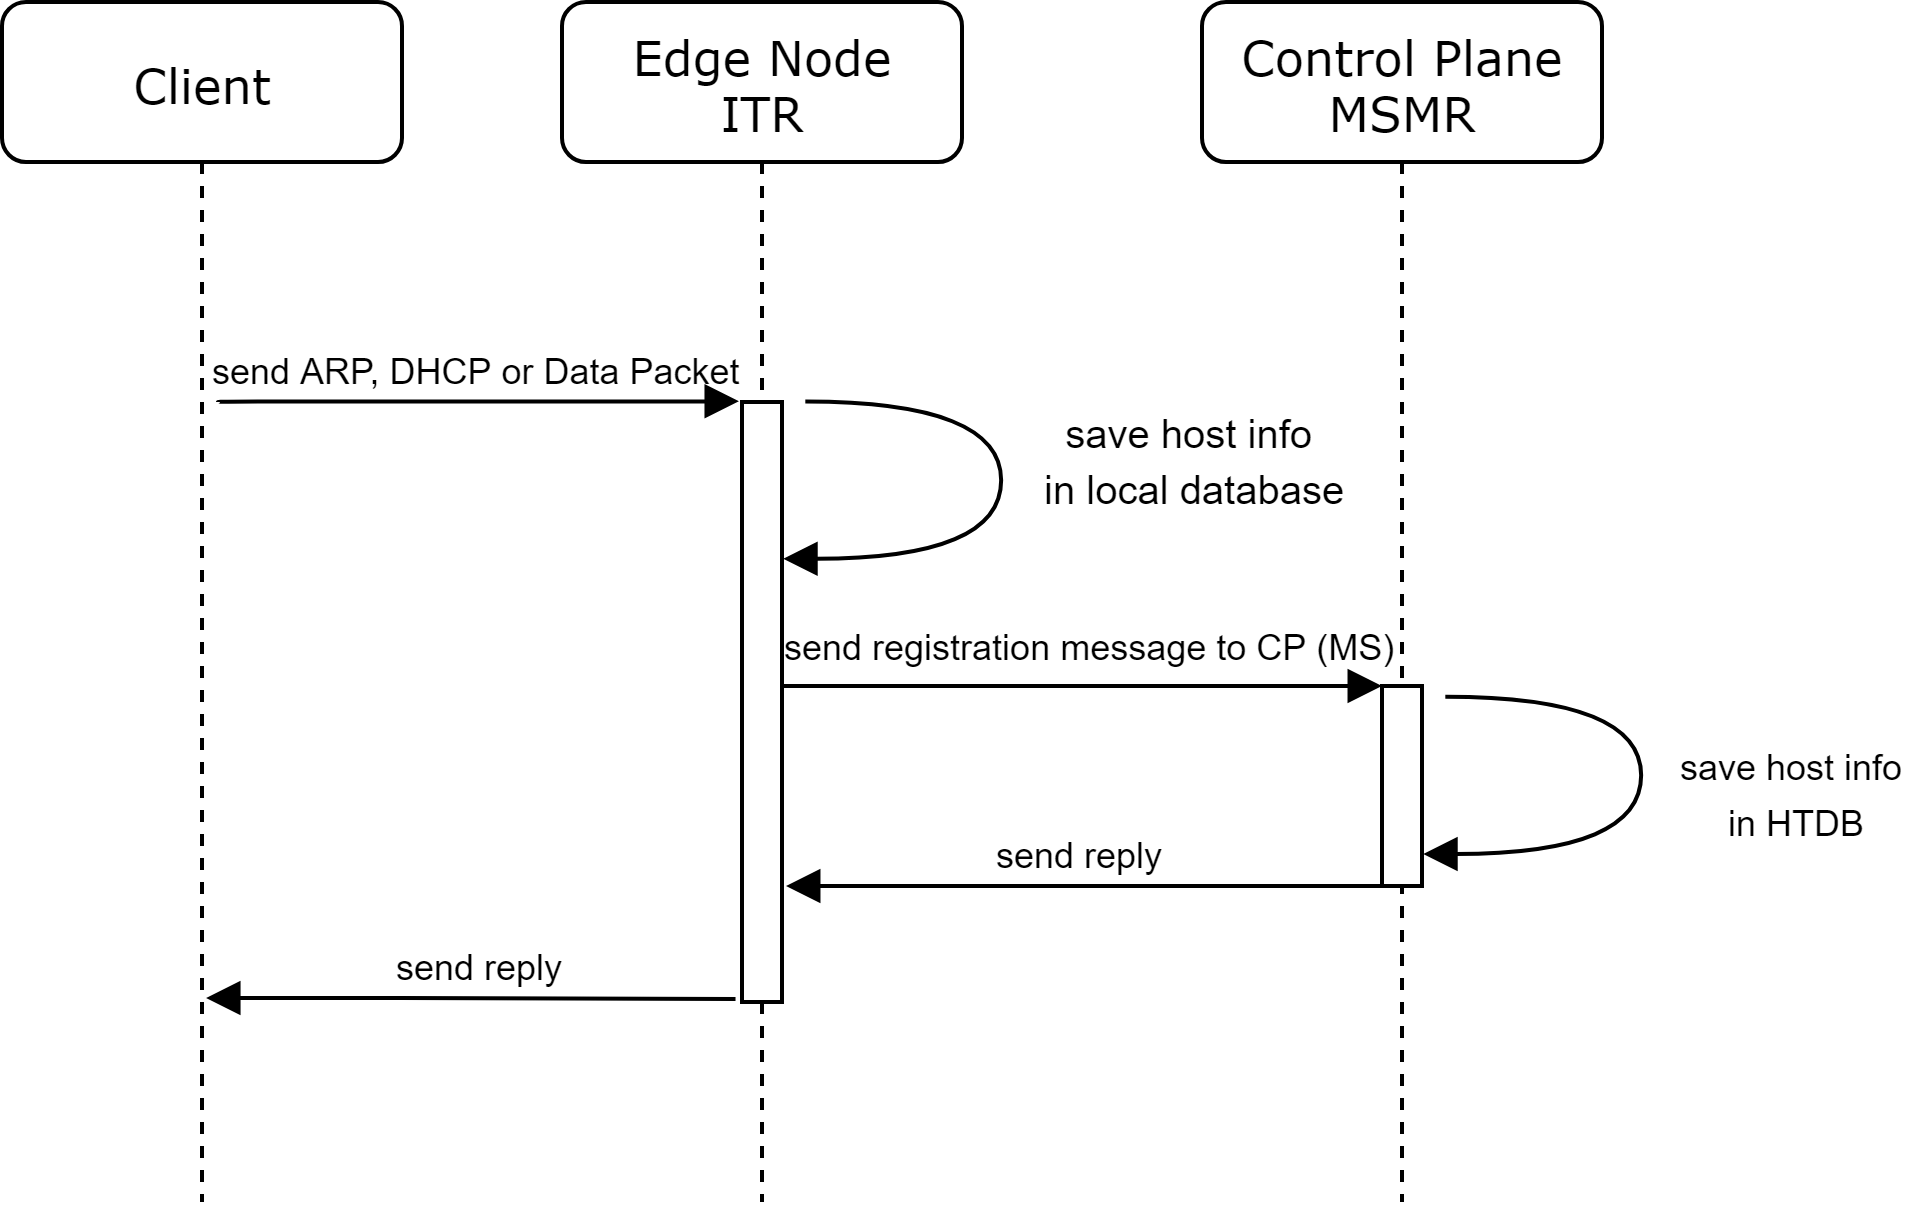
\includegraphics[width=0.8\linewidth]{img/Absicherung/LISP-ClientRegistration}
	\caption{LISP Client Registration}
	\label{fig:LISP Client Registration}
\end{figure}

\paragraph{LISP Host Resolution}
Will ein Client mit einem noch unbekannten anderen Client kommunizieren, so sucht sein ITR zuerst in seinem lokalen Map-Cache nach einem Eintrag. Ist noch kein Eintrag zum Client2 vorhanden, so schickt der ITR ein Map-Request zu seinem MR. Der MS sendet dann den originalen Map-Reguest an den zuletzt registrierten ETR. Da Client2 noch am ETR angeschlossen ist, sendet dieser einen Map-Reply an den ITR, welcher die angefragten Mapping-Informationen enthält.

Bei einem Ping werden die initialen Pakete verworfen, bis die Host Resolution abgeschlossen ist. 

\begin{figure}[H]
	\centering
	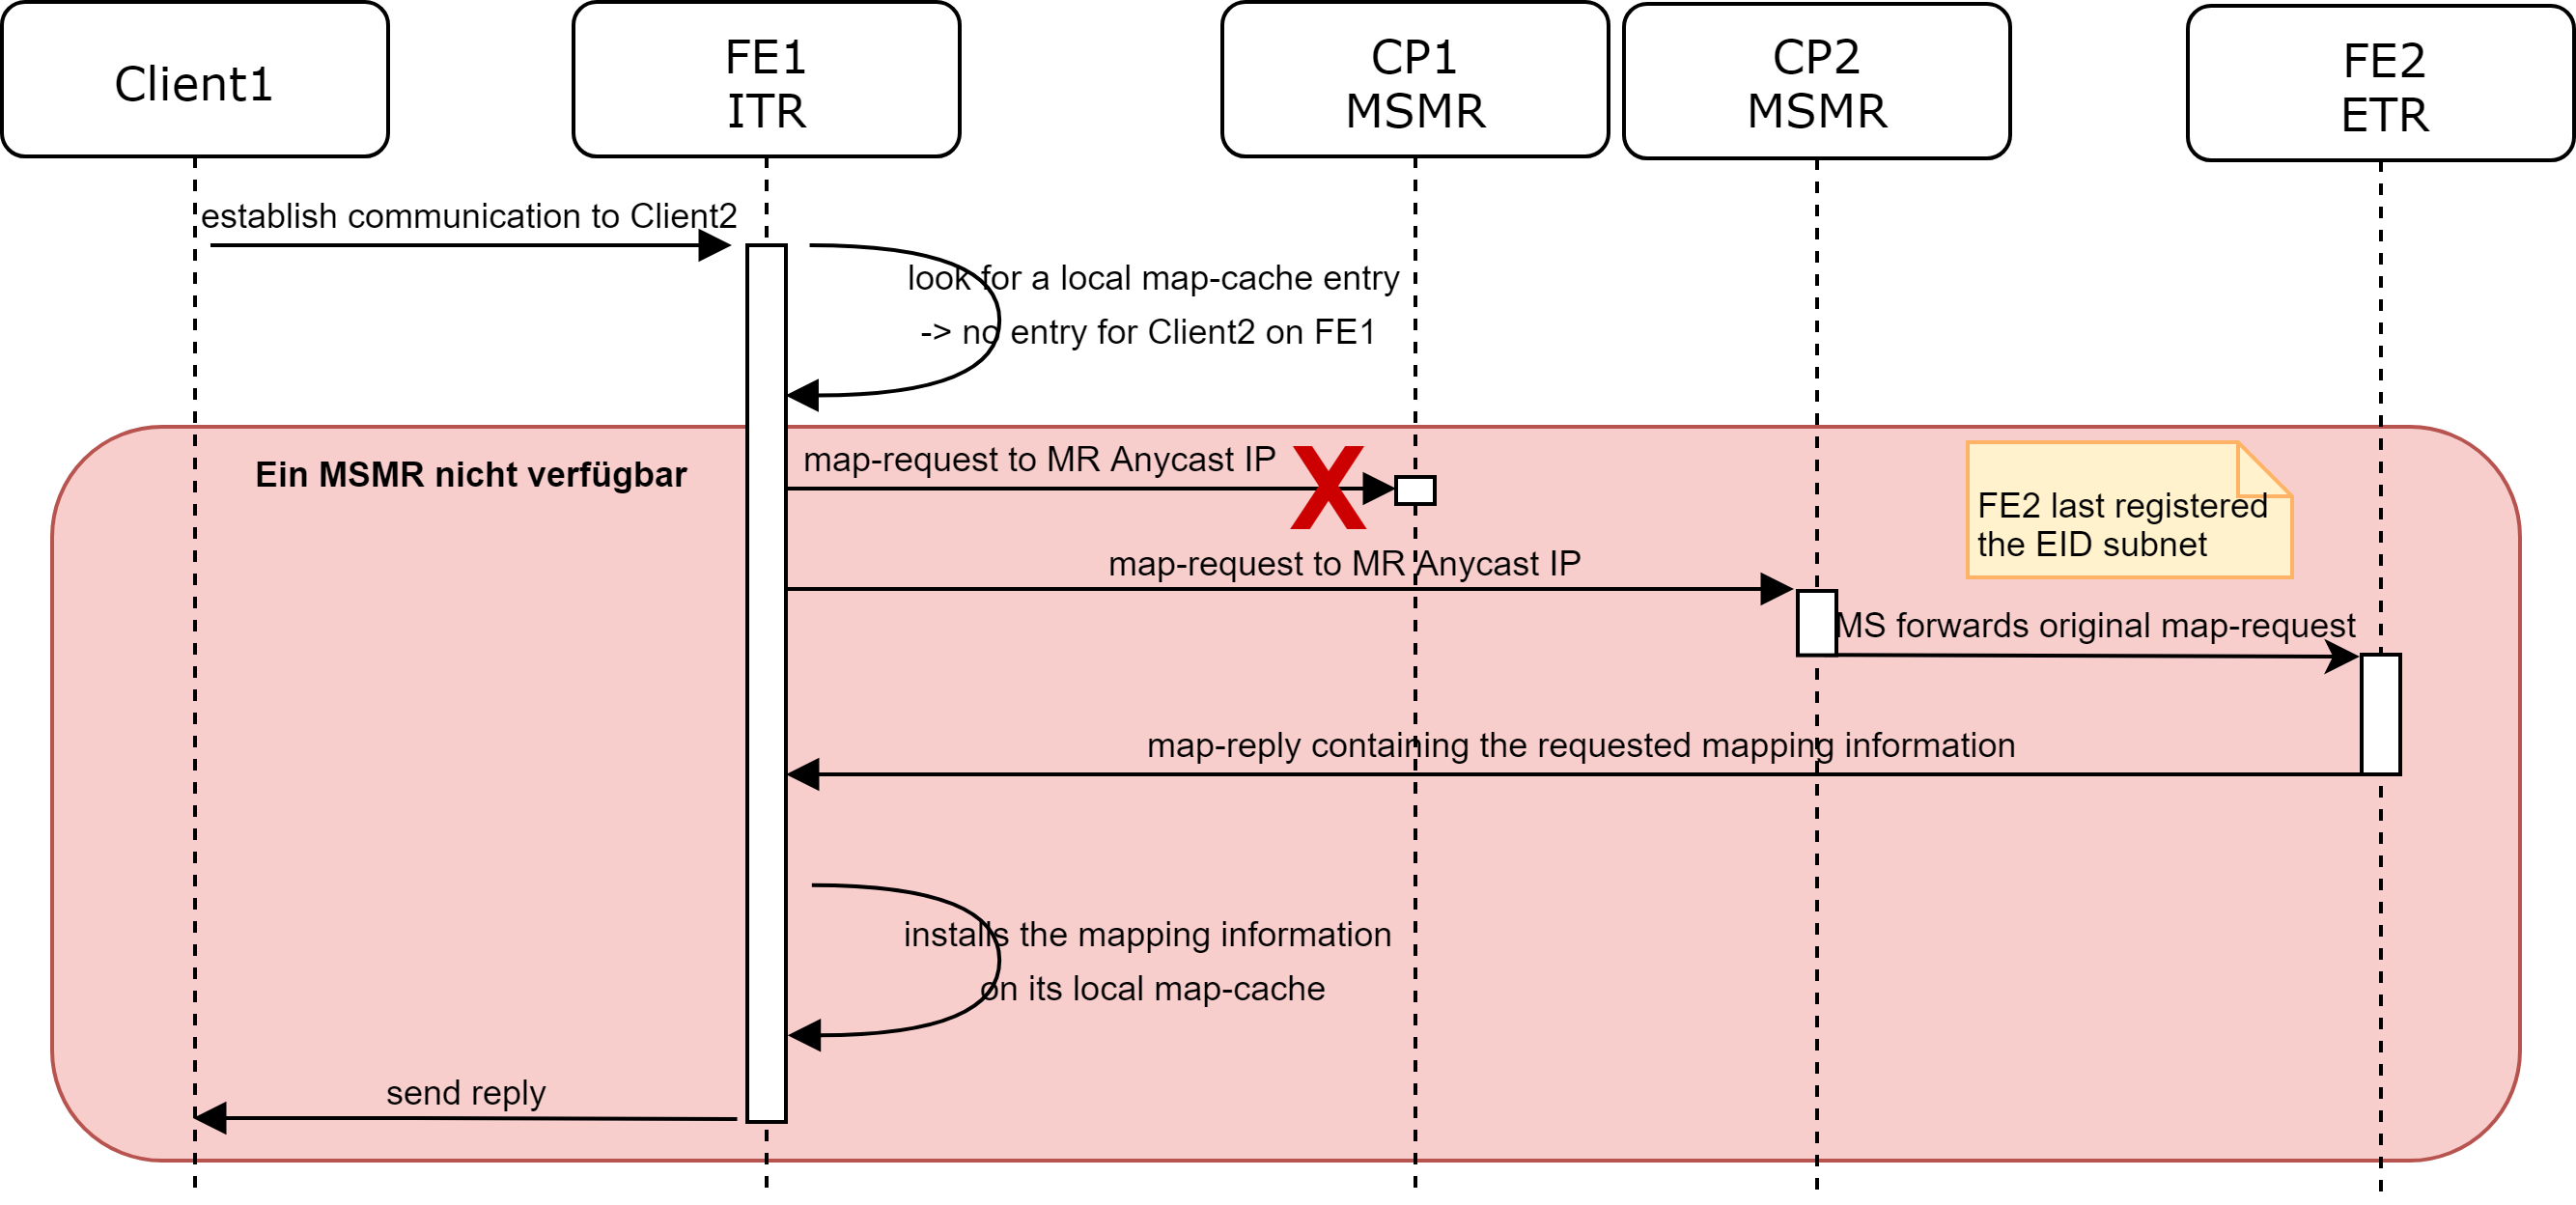
\includegraphics[width=1\linewidth]{img/Absicherung/LISP-HostResolution-Fail}
	\caption{LISP Host Resolution}
	\label{fig:LISP Host Resolution}
\end{figure}

\paragraph{Host Mobility}
Die Host Mobility ist ähnlich wie die Client Registration, da der Client sich beim neuen FE2 zuerst registriert und die neuen Informationen schliesslich vom CP1 dann an den alten FE1 zur Aktualisierung weitergegeben werden.

\begin{figure}[H]
	\centering
	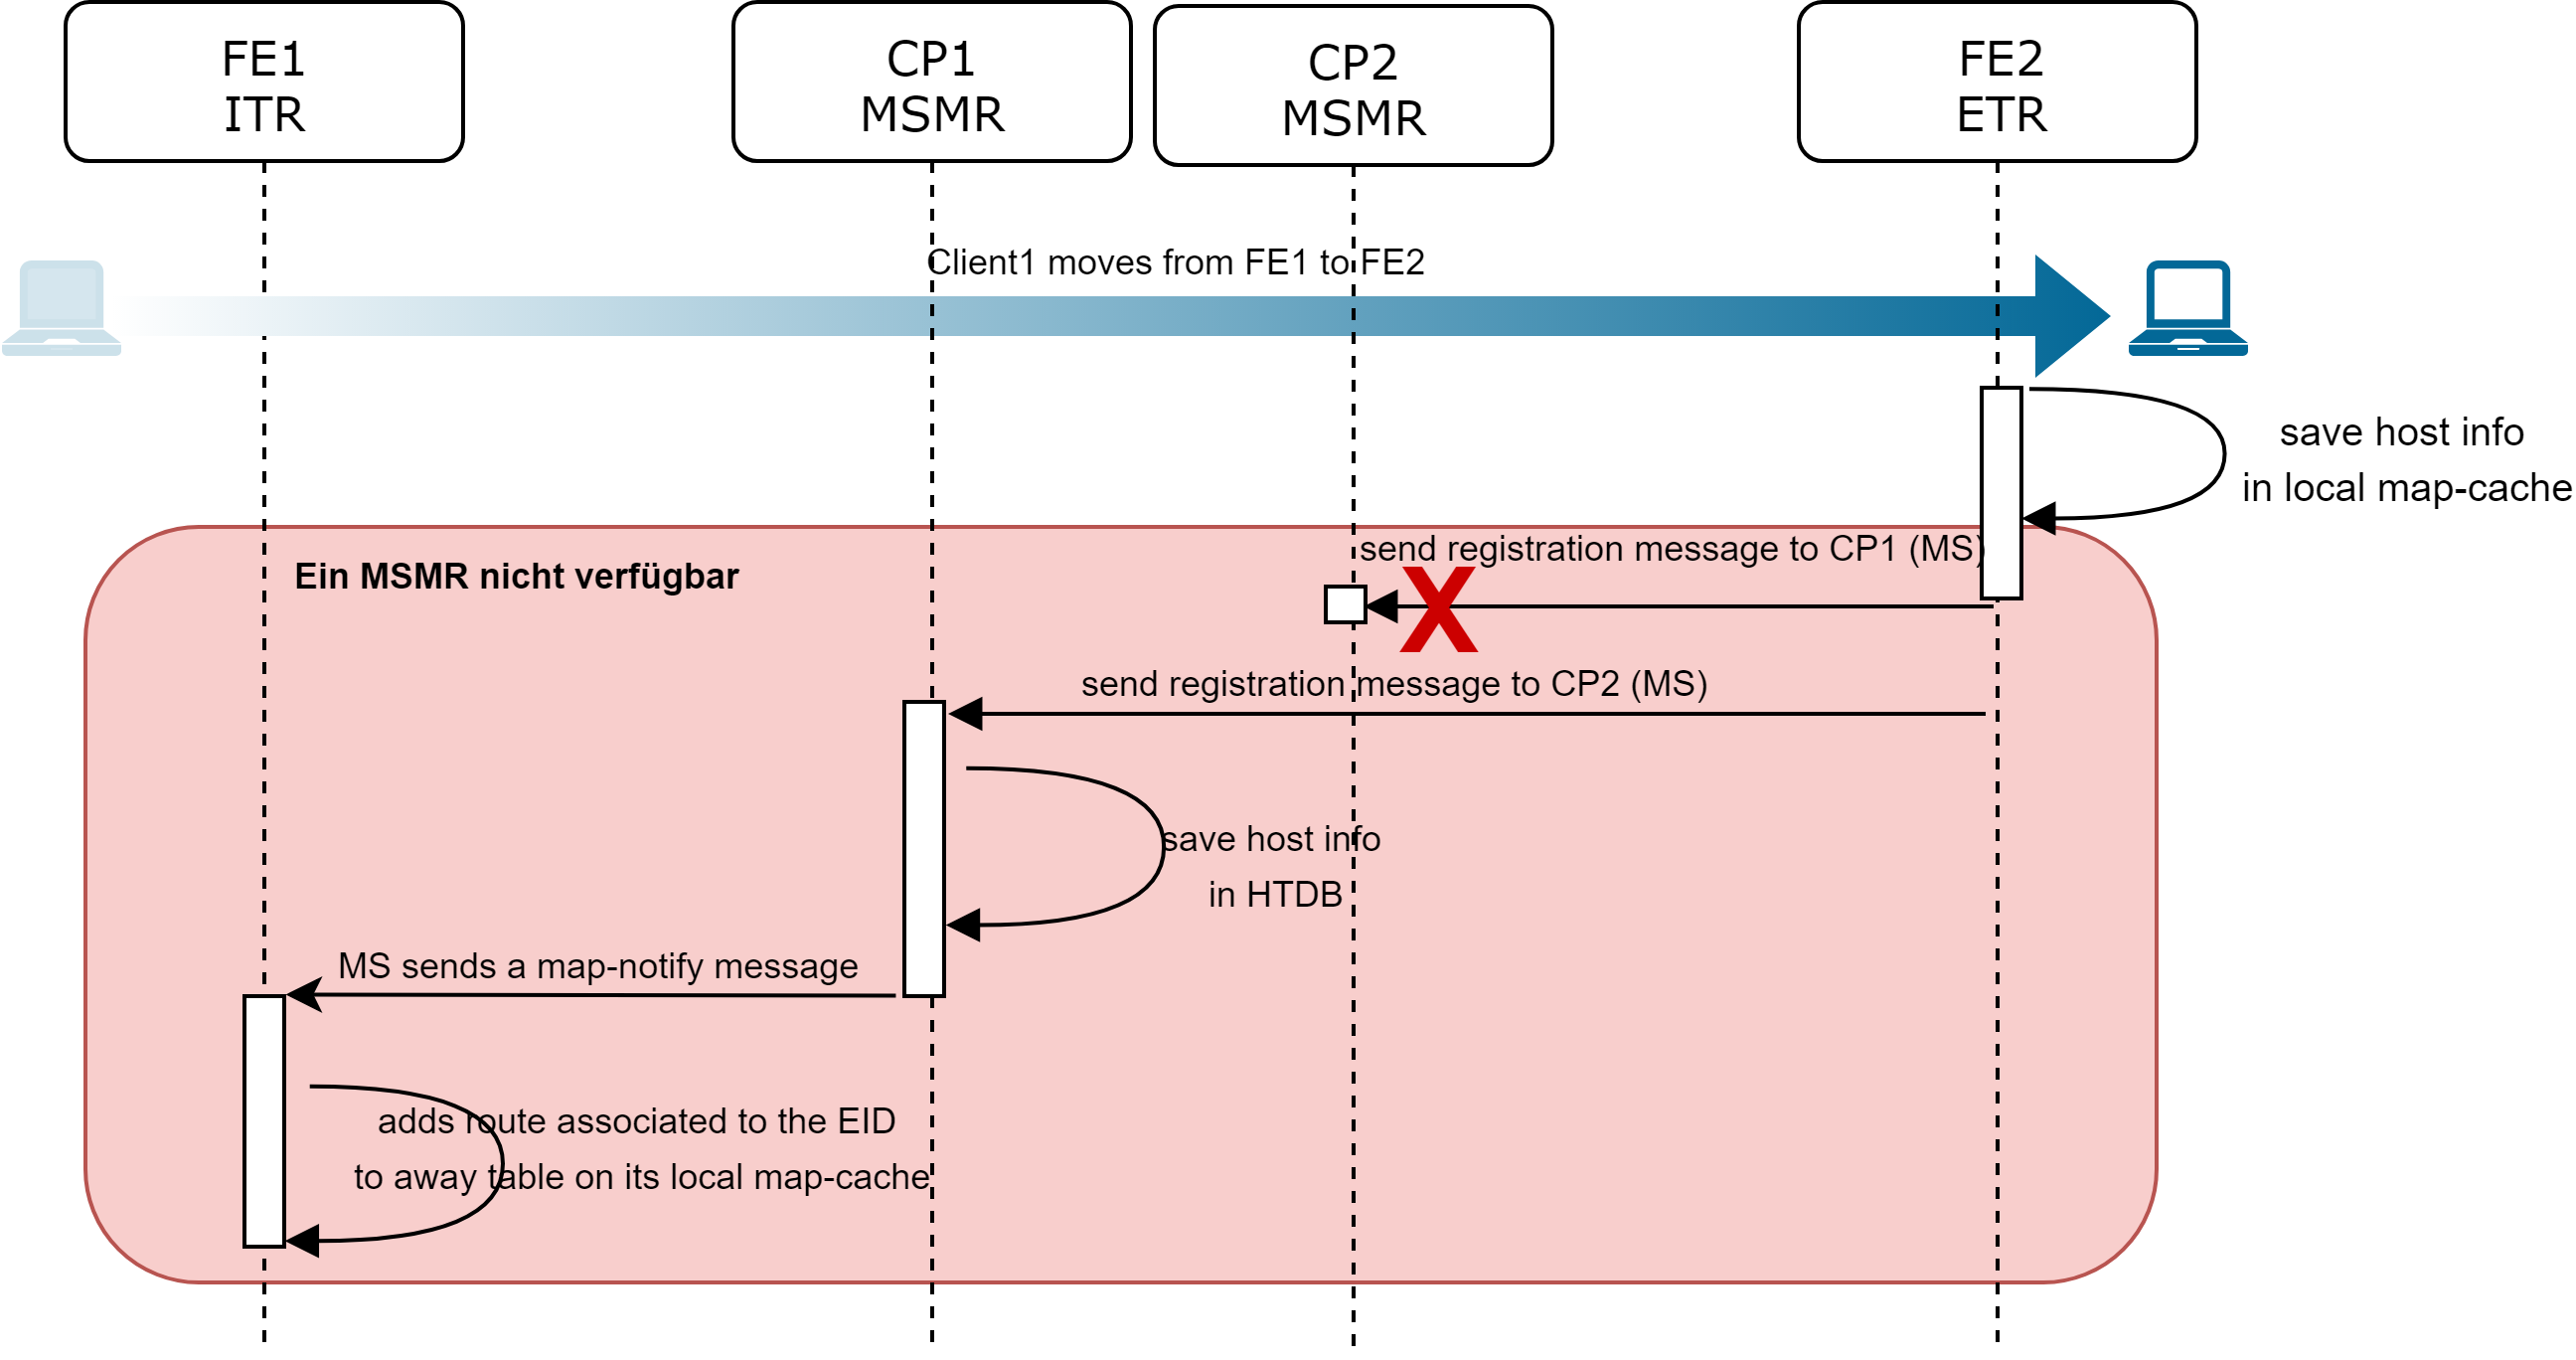
\includegraphics[width=1\linewidth]{img/Absicherung/LISP-HostMobility-Fail}
	\caption{LISP Host Mobility}
	\label{fig:LISP Host Mobility}
\end{figure}

Wenn ein dynamischer EID zwischen Rechenzentrumsstandorten wechselt, müssen die lokalen LISP Host Mobility-xTRs ihre Existenz erkennen. 

Das für LISP Host Mobility konfigurierte xTR erkennt ein Host Mobility Ereignis wenn:
\begin{enumerate}
	\item Er empfängt ein IP-Datenpaket von einer Quelle (des neu eingetroffenen Workloads), die aus Routing-Sicht nicht über die Schnittstelle erreichbar ist, auf der das Paket empfangen wurde.
	\item Die Quelle entspricht der auf die Schnittstelle angewendeten Dynamic-EID-Konfiguration.
\end{enumerate}


\subsubsection{Ausfall MSMR}
Bei einem Ausfall des MSMR kann keine Host Registration mehr vorgenommen werden. Das heisst neue Clients können keine Verbindung zum restlichen Netzwerk aufbauen. Bestehende Clients können nur mit Clients welche am selben FE angeschlossen sind kommunizieren. Dies jedoch nur solange ihr Eintrag im lokalen Map-Cache bestehen bleibt. Der TTL der Einträge im Map-Cache beträgt per default einen Tag. 

Da jeder xTR seinen eigenen Map-Cache hat und kann sich sein Inhalt innerhalb derselbe LISP-Site unterscheiden. Daher können xTr leicht schwere Paketausfälle erleiden und mit LISP Control Messages geflutet werden.  

\paragraph{MS}
Es sollten mehrere Map-Server vorhanden und eingetragen sein. Optimalerweise ist mindestens ein Map-Server pro Site vorhanden. Sollte der erste Map-Server nicht erreichbar sein, so wird der zweite Map-Server verwendet.

\paragraph{MR}
Für den Map-Resolver sollte eine Anycast IP-Adresse verwendet werden. So werden die Pakete gesendet und über einen verfügbaren Map-Resolver zum Ziel weitergeleitet. Auch hier ist es sinnvoll, mindestens einen Map-Resolver pro Site bereitzustellen.

\subsubsection{Analyse mittels LISP Commands}
Es gibt viele LISP Befehle, welche die Analyse vereinfachen können. Nachfolgend zeigen wir einige LISP Commands, zusammen mit den ihren Ausgaben. \cite{lisp-commands}

\paragraph{LISP EID-Table}
Auf einem Control Plane kann die EID-Tabelle mit folgendem Befehl ausgegeben werden:

\begin{lstlisting}[language=bash]
show lisp eid-table vrf <VRF Name> ipv4 map-cache
\end{lstlisting}


\begin{figure}[H]
	\centering
	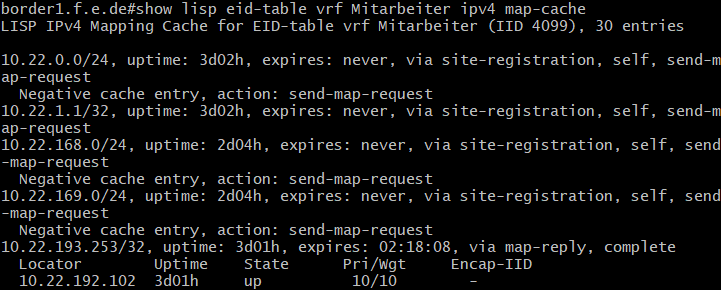
\includegraphics[width=0.8\linewidth]{img/Absicherung/lisp_eid-table}
	\caption{LISP EID-Table}
	\label{fig:LISP EID-Table}
\end{figure}




\paragraph{LISP EID-Table Map Cahe Entry}
Ein Eintrag in der EID-Table im Map Cache kann mit folgender Abfrage detaillierter angezeigt werden:

\begin{lstlisting}[language=bash]
show lisp eid-table vrf <VRF Name> ipv4 map-cache <IP>
\end{lstlisting}


\begin{figure}[H]
	\centering
	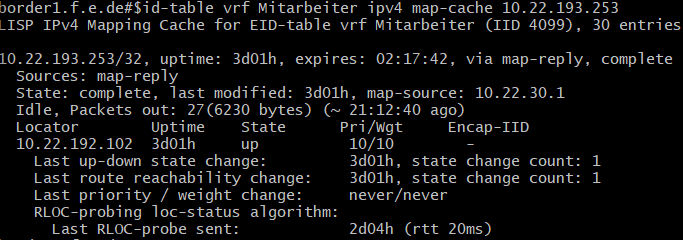
\includegraphics[width=0.8\linewidth]{img/Absicherung/lisp_eid-table-entry}
	\caption{LISP EID-Table Map Cache Entry}
	\label{fig:LISP EID-Table Map Cache Entry}
\end{figure}

\paragraph{LISP Database EID-Table}
Der folgende Befehl kann verwendet werden, um die Egress Tunnel Router (ETR) konfigurierten lokalen IPv4-EID-Präfixes und der zugehörigen Locator-Sets auszugeben:

\begin{lstlisting}[language=bash]
show ip lisp database eid-table <VRF Name>
\end{lstlisting}

\begin{figure}[H]
	\centering
	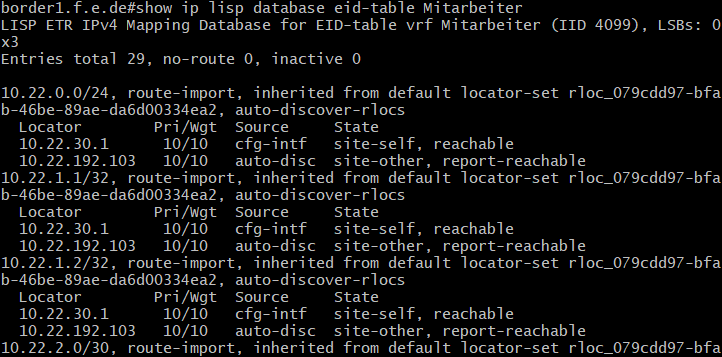
\includegraphics[width=0.8\linewidth]{img/Absicherung/lisp_eid-table-database-rloc}
	\caption{LISP Database EID-zu-RLOC}
	\label{fig:LISP Database EID-zu-RLOC}
\end{figure}






\subsection{ISE / Radius / SGT}

\subsubsection{Deployment Size and Scaling Recommendations}

Die nachfolgenden Tabellen zeigen die Performance und Scalability Metriken für Radius Sessions, Passive Identity, Easy Connect, pxGrid und ISE Services.

\begin{figure}[H]
	\centering
	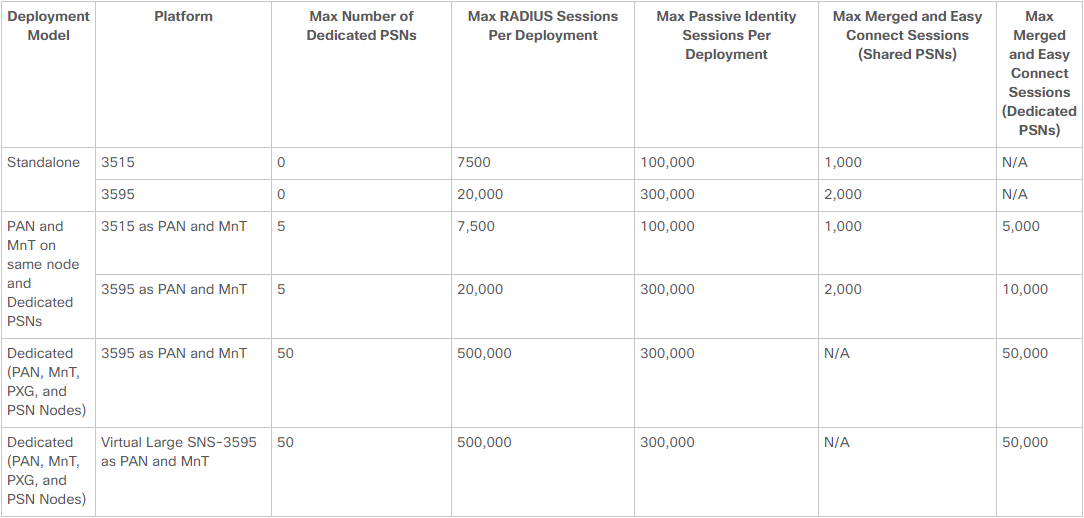
\includegraphics[width=1\linewidth]{img/Absicherung/ISE-MaxRadiusScaling}
	\caption{ISE - Maximum RADIUS Scaling by Deployment with Maximum Passive Identity/Easy Connect Scaling by Deployment Size \cite{ise-scale}}
	\label{fig:ISE - Maximum RADIUS Scaling}
\end{figure}

\begin{figure}[H]
	\centering
	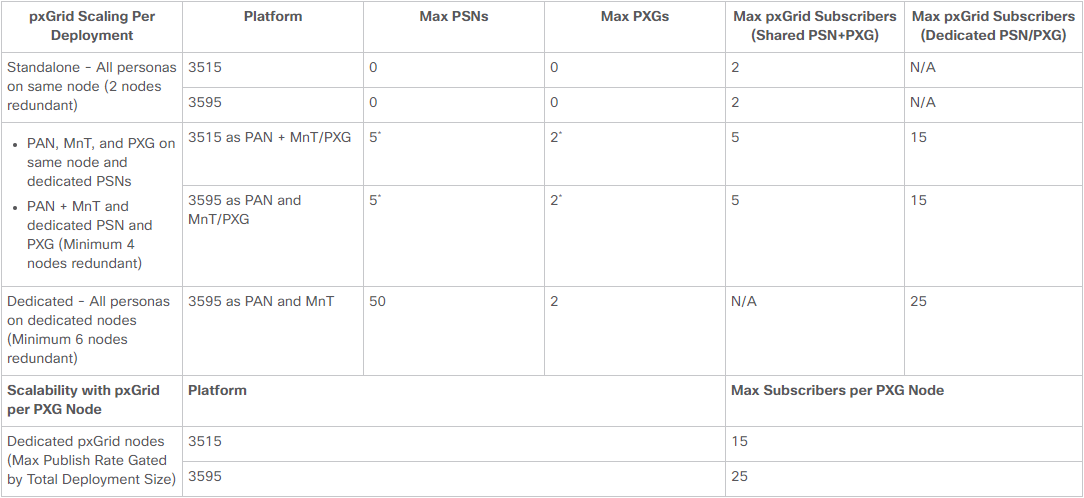
\includegraphics[width=1\linewidth]{img/Absicherung/ISE-pxGridServicesScalability}
	\caption{ISE - Scalability with pxGrid Services \cite{ise-scale}}
	\label{fig:ISE - Scalability with pxGrid Service}
\end{figure}

\begin{figure}[H]
	\centering
	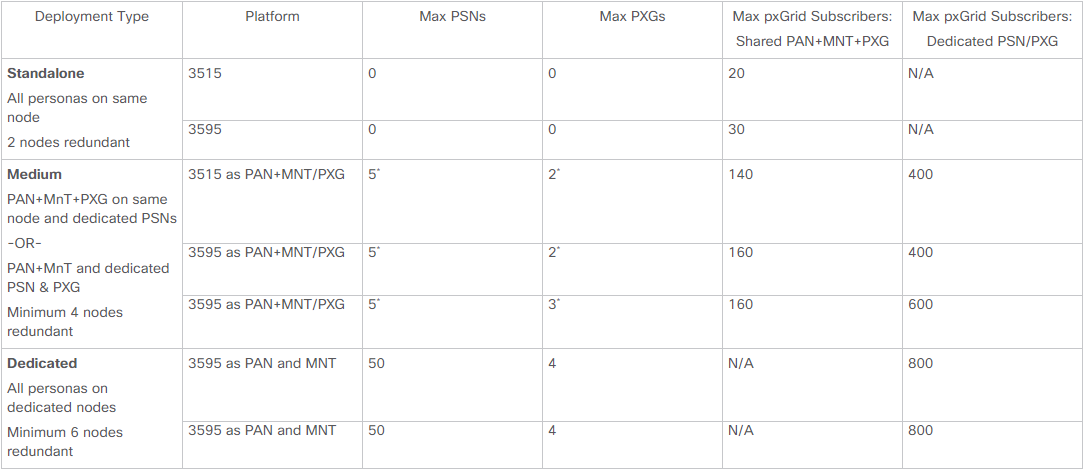
\includegraphics[width=1\linewidth]{img/Absicherung/ISE-PlatformpxGridV2Scaling}
	\caption{ISE - pxGrid v2 Scaling per Dedicated pxGrid Node \cite{ise-scale}}
	\label{fig:ISE - pxGrid v2 Scaling per Dedicated pxGrid Node}
\end{figure}

\begin{figure}[H]
	\centering
	\includegraphics[width=0.5\linewidth]{img/Absicherung/ISE-pxGridV2}
	\caption{ISE - Platform eXchange Grid (pxGrid v2) Scaling \cite{ise-scale}}
	\label{fig:ISE - Platform eXchange Grid (pxGrid v2) Scaling}
\end{figure}

\subsubsection{ISE Cluster}

Um die Verfügbarkeit des ISE zu erhöhen, kann diese in einem Cluster, bestehend aus einem Primary Node und einem Secondary Node, betrieben werden. Dies erhöht die Ausfallsicherheit aller Services auf dem ISE.

\subsubsection{Distributed Deployment}

Damit Aussenstandorte auch gegen einen Ausfall der Verbindung zum Hauptstandort abgesichert sind, macht ein Distributed Deployment Sinn. Dies bedeutet, dass an jedem Standort mindestens ein ISE Server betrieben wird. 

\begin{figure}[H]
	\centering
	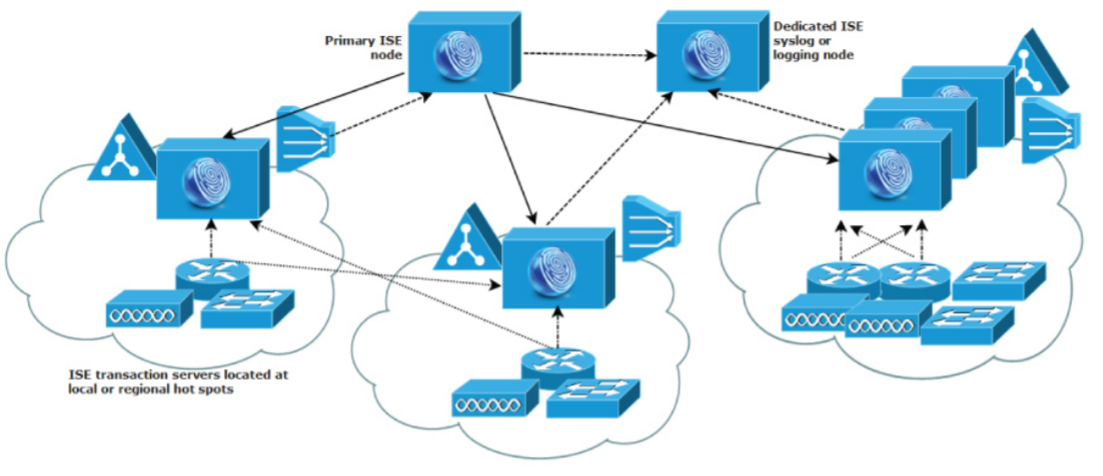
\includegraphics[width=0.8\linewidth]{img/Absicherung/ISE-Distributed-Deployment.png}
	\caption{ISE - Distributed Deployment \cite{ise-install-guide}}
	\label{fig:ISE - Distributed Deployment}
\end{figure}

Alle Informationen des Primary Node werden auf die Secondary Nodes an den Aussenstandorten repliziert. Network Access Devices und Clients an diesen Standorten können also die lokale Instanz verwenden.  Für wichtige Standorte kann die Ausfallsicherheit und Performance weiter erhöht werden, indem dort mehrere Instanzen betrieben werden.

\paragraph{Installation auf dem ENCS 5400}

Die Installation des ISE auf dem ENCS 5400 funktioniert ähnlich, wie dies bereits in Kapitel 4.2 beschrieben wurde. Daher werden hier nur die Besonderheiten des ISE beschrieben.

\subparagraph{Image Upload}
Für den ISE kann kein komplettes Disk Image importiert werden. Daher wird in diesem Fall das ISO auf den ENCS kopiert. Auf Grund der Grösse des ISOs kann dies aber nicht über das Web-Interface gemacht werden.

\begin{figure}[H]
	\centering
	
\includegraphics[width=0.8\linewidth]{img/Absicherung/ENCS-Upload-Limit.png}
	\caption{ENCS - Upload Limit}
	\label{fig:ENCS - Upload Limit}
\end{figure}

Ein Image oder ISO über 6GB muss daher via USB, SCP oder NFS auf den ENCS kopiert werden. 

\begin{lstlisting}[language=bash]
nfvis# scp root@10.22.0.15:/root/isos/ise-2.3.iso intdatastore:
\end{lstlisting}

Nach dem Upload muss das ISO noch registriert werden. \textit{VM Life Cycle $\rightarrow$ Image Repository $\rightarrow$ Browse Datastore $\rightarrow$ Register}

\subparagraph{Image Deployment}

Falls noch kein passendes Profil existiert, muss dieses wie in Kapitel 4 beschrieben erstellt werden. Hierbei sind die sehr hohen Hardwareanforderungen der ISE zu beachten. Die bei uns verwendete Version 2.3 stellt folgende Anforderungen:

\begin{table}[H]
	\rowcolors{2}{gray!25}{white}
	\centering
	\begin{tabularx}{\textwidth}{l | X}
		CPU & 4 Cores mit je 1.8 GHz        \\
		\hline
		Memory & 6GB \\
		\hline
		Hard Disk & 100 GB (Write IO 50MB/s, Read IO 300MB/s) \\
	\end{tabularx}
	\caption{ISE Requirements}
	\label{tab:ISE Requirements}
\end{table}

Die VM kann nun unter \textit{VM Life Cycle $\rightarrow$ Deploy} erstellt werden. Es wird eine VM vom Typ \textit{OTHER} benötigt. Es muss ein Name, das Image und ein Profil definiert werden. Zudem muss die VM mit allen nötigen Netzwerken verbunden werden.

\begin{figure}[H]
	\centering
	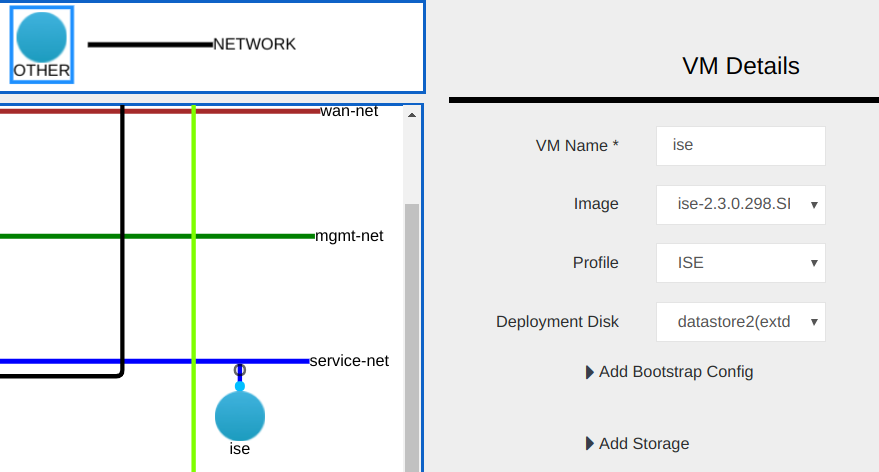
\includegraphics[width=0.8\linewidth]{img/Absicherung/ENCS-ISE-Deployment.png}
	\caption{ENCS - ISE Deployment}
	\label{fig:ENCS - ISE Deployment}
\end{figure}

\subparagraph{ISE Konfiguration}

Sobald die VM deployed ist, wird das Setup gestartet. Es müssen grundlegende Informationen wie Hostname und Netzwerkeinstellungen konfiguriert werden.  

\begin{figure}[H]
	\centering
	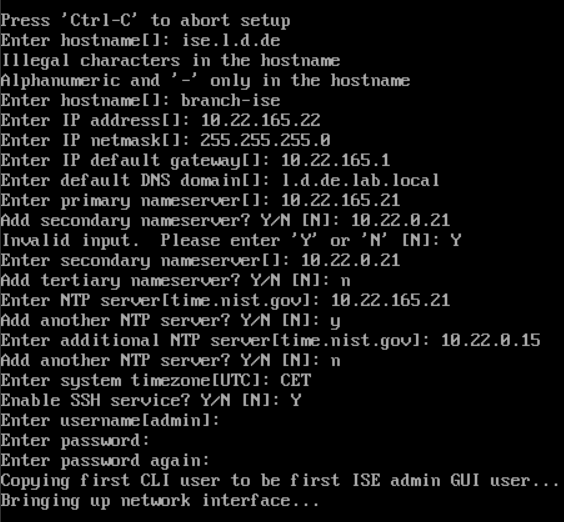
\includegraphics[width=0.8\linewidth]{img/Absicherung/ISE-Setup.png}
	\caption{ISE-Setup}
	\label{fig:ISE-Setup}
\end{figure}

\subparagraph{Distributed Deployment}

Sobald die Installation des zweiten Nodes abgeschlossen ist, kann diese auf dem Primary Node als Secondary Node hinzugefügt werden.

TODO

\subsubsection{Third Party Software}

Alternativ zum Distributed Deployment der ISEs kann eine Replikation der Services auch mittels Third Party Software erreicht werden. 

\subsubsection{Read Only Radius Server an Aussenstandorten}

In Aussenstellen wird ein Read Only Radius Server betrieben, damit die Network Access Devices auch im Falle eines Unterbruchs der Verbindung zum Hauptsitz einen Radius Server zur Verfügung haben. Hier könnte beispielsweise Freeradius eingesetzt werden. Da Freeradius seine Informationen nicht direkt vom ISE beziehen kann, muss vom ISE ein externer Radius Server verwendet werden, der eine Replikation unterstützt. 


\paragraph{ISE}
An einem Hauptstandort wird der primäre ISE Node und ein Dedicated ISE Syslog oder Logging Node betrieben. In einem grossen zentralisierten Netzwerk sollte ein Load Balancer verwendet werden, der die Bereitstellung von AAA-Services vereinfacht. Die Verwendung eines Load Balancers erfordert nur einen einzigen Eintrag für die AAA-Server und der Load Balancer optimiert das Routing von AAA-Anfragen an die verfügbaren Server. Um einen Single Point of Failure zu vermeiden, sollten zwei Load Balancer mit Failover IP eingesetzt werden.

Weitere verteilte grosse Standorte können über eine eigene AAA-Infrastruktur für eine optimale AAA-Performance verfügen. Ein zentralisiertes Verwaltungsmodell hilft bei der Aufrechterhaltung einer konsistenten, synchronisierten AAA-Richtlinie. Ein zentralisiertes Konfigurationsmodell verwendet einen primären Cisco ISE Node mit einem sekundären Cisco ISE Node. 

\paragraph{Freeradius}

Freeradius wird in einem Master / Slave Setup betrieben. Am Hauptstandort befindet sich der Radius Master und an allen Aussenstandorten ist ein Slave verfügbar. Die Replikation wird mittels MySQL Replikation sichergestellt.

\paragraph{Network Access Devices}

Auf den Network Devices muss der Radius Server vom jeweiligen Standort konfiguriert sein. Dies kann im DNA Center unter \textit{Design $\rightarrow$ Network Settings $\rightarrow$ AAA Server} konfiguriert werden.

\begin{figure}[H]
	\centering
	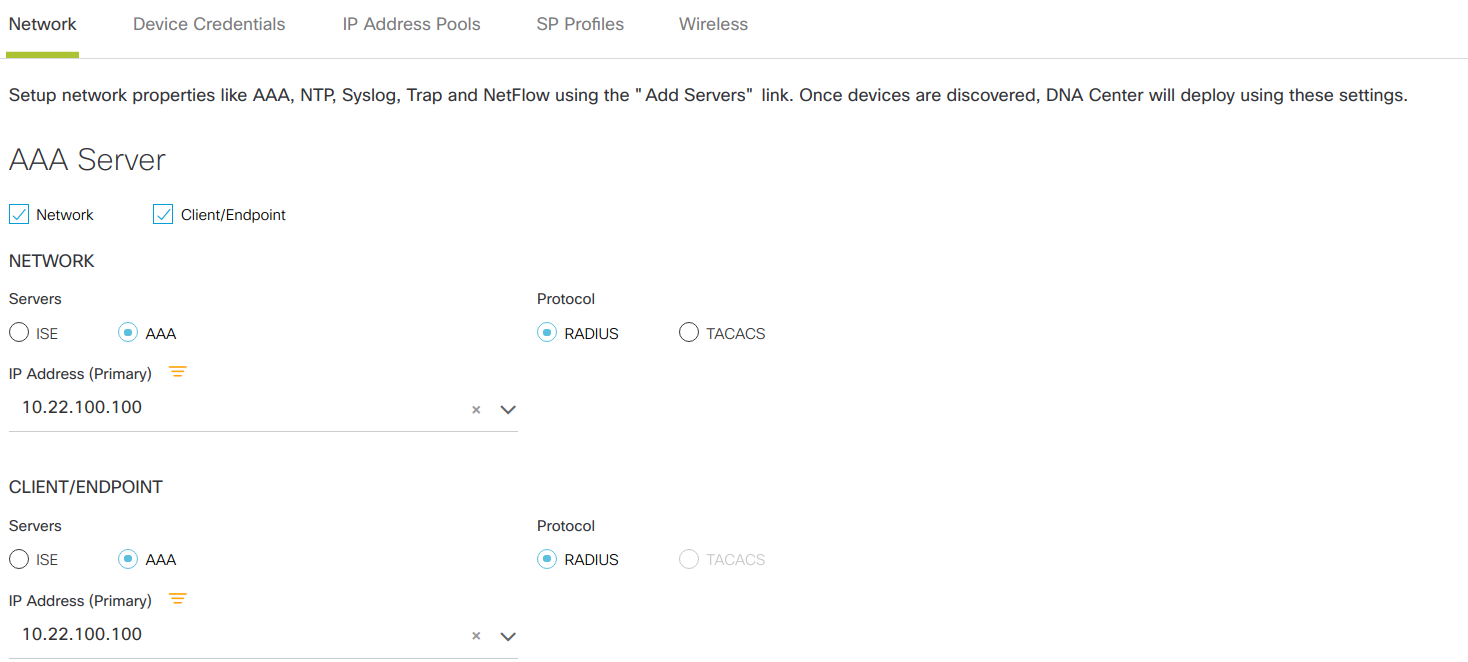
\includegraphics[width=0.8\linewidth]{img/Absicherung/DNA_Center_AAA-Server.png}
	\caption{DNA Center - AAA Server }
	\label{fig:DNA Center - AAA Server}
\end{figure}


\subsection{SGT Access List}
Beim Erstellen von SGTs über die DNAC-Benutzeroberfläche wird auf die ISE-Benutzeroberfläche weitergeleitet und die Aufgabe wird dort abgeschlossen. ISE verwaltet alle Gruppeninformationen, die später in DNAC für die Richtlinienerstellung verwendet werden. Obwohl die Richtlinien und die entsprechenden Contracts bei DNAC erstellt werden, werden beide über die REST-API der ISE an die ISE zurückgemeldet. ISE dient dann als zentrale Anlaufstelle für SGTs, Richtlinien und SGACLs, die dann dynamisch an die Netzwerkinfrastruktur verteilt werden.
Die Segmentierung innerhalb der SDA wird durch die kombinierte Verwendung von virtuellen Netzwerken (VN), die mit VRFs gleichgesetzt sind, als auch TrustSec Scalable Group Tags (SGTs) ermöglicht. Während die Segmentierung durch die Verwendung von absichtsgesteuerten oder speziell dafür entwickelten virtuellen Netzwerken allein erreicht werden kann, bieten die Cisco Trustsec SGTs eine logische Segmentierung basierend auf der Gruppenmitgliedschaft. Cisco bietet eine zusätzliche Granularitätsebene, mit der mehrere SGTs innerhalb eines einzigen VN verwenden können, die eine Mikrosegmentierung innerhalb des VN ermöglicht. Die Segmentierung erfolgt innerhalb des SDA sowohl auf Makro- als auch auf Mikroebene durch virtuelle Netzwerke bzw. SGTs. Die Richtlinien und die damit verbundenen Contracts werden im DNAC konfiguriert und dann über die REST-API an die ISE übermittelt. ISE aktualisiert dann die Edge Nodes mit den Richtlinien für SGTs, die den angeschlossenen Geräten zugeordnet sind. 
\cite{sda-segmentation-may2018}

Kurze Zusammenfassung der damit benötigten Komponenten:
\begin{itemize}
	\item Sicherheitsgruppe (SG) - Eine Gruppe von Benutzern, Endpunktgeräten und Ressourcen, die Zugriffssteuerungsrichtlinien gemeinsam nutzen. SGs werden vom Administrator in Cisco ISE definiert. Wenn neue Benutzer und Geräte zur TrustSec Domäne hinzugefügt werden, ordnet Cisco ISE diese neuen Entitäten den entsprechenden Sicherheitsgruppen zu.
	\item Security Group Tag (SGT) - Der TrustSec-Dienst weist jeder Sicherheitsgruppe eine eindeutige 16-Bit-Sicherheitsgruppennummer zu, deren Gültigkeitsbereich innerhalb einer TrustSec Domäne global ist. Die Anzahl der Sicherheitsgruppen im Switch ist auf die Anzahl der authentifizierten Netzwerkentitäten beschränkt. Die Sicherheitsgruppennummern müssen nicht manuell konfigurieren. Sie werden automatisch generiert, aber es gibt auch die Möglichkeit eine Reihe von SGTs für die IP-zu-SGT-Zuordnung zu reservieren.
	\item Security Group Access Control List (SGACL) - Mit SGACLs kann der Zugriff und die Berechtigung basierend auf den zugewiesenen SGTs gesteuert werden. Die Gruppierung von Berechtigungen in einer Rolle vereinfacht die Verwaltung von Sicherheitsrichtlinien. Beim Hinzufügen von Geräten wird einfach eine oder mehrere Sicherheitsgruppen zugewiesen und diese erhalten sofort die entsprechenden Berechtigungen. Die Sicherheitsgruppen können geändert werden, um neue Berechtigungen einzuführen oder die aktuellen Berechtigungen einzuschränken.
	\item Security Exchange Protocol (SXP) - Das SGT Exchange Protocol (SXP) ist ein Protokoll, das für den TrustSec Dienst entwickelt wurde, um die IP-SGT-Bindungen auf Netzwerkgeräte zu übertragen, die keine SGT-fähige Hardwareunterstützung für Hardware bieten, die SGT / SGACL unterstützt.
\end{itemize}

\begin{figure}[H]
	\centering
	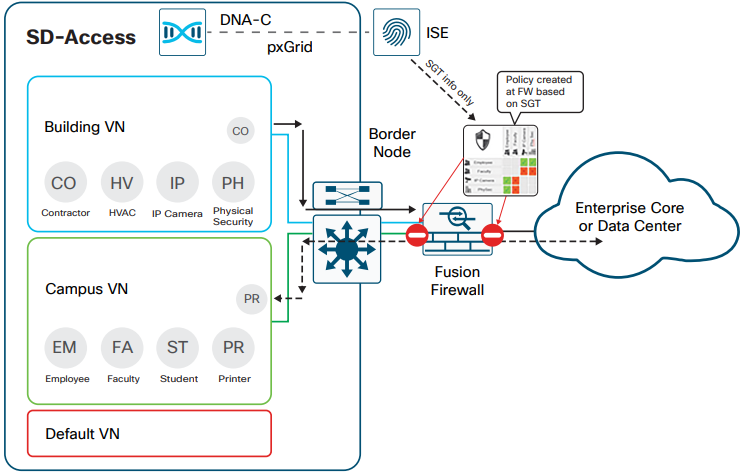
\includegraphics[width=1\linewidth]{img/Absicherung/SGT-FusionFirewall}
	\caption{Policy Enforcement mit einer Fusion Firewall}
	\label{fig:Policy Enforcement mit einer Fusion Firewall}
\end{figure}

Die obige Abbildung veranschaulicht die Verwendung einer Fusion Firewall, welche für die Kommunikation zwischen virtuellen Netzwerken sowie für den Verkehr an einem anderen Ort im Netzwerk. Mit Hilfe von Standard ACLs oder gruppenbasierten Richtlinien mit SGTs werden Firewall-Regeln in der Fusions-Firewall definiert, die den Datenverkehr zwischen Endpunkten steuert.

\subsubsection{Failover}
Die Absicherung der Access Listen kann beispielsweise nach folgenden Beispielen erarbeitet werden:

\begin{itemize}
	\item Beispiel1: lokal auf 9300 SGACLs alle fünf Minuten sichern und diese bei Ausfall wieder eintragen. Nachteil: Host-Mobility funktioniert nicht, aber lokal kann weitergearbeitet werden.
	\item Beispiel2: global komplett alle SGACLs auf alle Geräte verteilen. Vorteil: Alle Geräten haben jederzeit alle Einträge. Nachteil: Die Maximum Scale Recommendations der SGACLs sind pro Gerät anders. C3850 - 1500 SGACLs, C9300 - 5000 SGACLs
\end{itemize}

Es können TrustSec SXP Speaker/Listener auf den Catalyst 3850 und C9300 definiert werden, indem die Catalyst 3850 als Gateway für die Catalyst 9300 Listener angegeben werden.

\subsection{Border Node}

Der gesamte Verkehr der die Fabric betritt oder verlässt, durchläuft diesen Knoten. Um einen Single Point of Failure zu vermeiden, sollten immer mindestens zwei Border Nodes pro Site zur Verfügung stehen. Nach den aktuellen Maximum Scale Recommendations können maximal 4 Border Nodes Site implementiert werden.

Border Nodes implementieren die folgenden Funktionen, welche bei einem Ausfall in Mitleidenschaft gezogen werden könnten\cite{sda-designguide-sept2018}:
\begin{itemize}
	\item Ankündigung von EID-Subnetzen
	\item Fabric-Domänenausstiegspunkt
	\item Mapping der LISP-Instanz auf VRF
	\item Richtlinienzuordnung
\end{itemize}

\subsubsection{Ankündigung von EID-Subnetzten}
SD-Access konfiguriert Border Gateway Protocol (BGP) als bevorzugtes Routingprotokoll, das für die Ankündigung der EID-Präfixe außerhalb der Fabric verwendet wird, und der für EID-Subnetze von außerhalb der Fabric bestimmte Verkehr wird durch die Grenzknoten geleitet. Diese EID-Präfixe werden nur in den Routingtabellen am Rand angezeigt. Im gesamten Rest der Fabric wird auf die EID-Informationen über die Fabric-Steuerebene zugegriffen.

\subsubsection{Fabric-Domänenausstiegspunkt}
Der externe Fabric Border ist das Gateway des letzten Auswegs für die Fabric Edge Nodes. Dies wird mithilfe der LISP Proxy Tunnel Router-Funktionalität implementiert. Möglich sind auch interne Fabric Borders, die mit Netzwerken mit einem genau definierten Satz von IP-Subnetzen verbunden sind, wodurch die Ankündigung dieser Subnetze in der Fabric hinzugefügt werden muss.

\subsubsection{Mapping der LISP-Instanz auf VRF}
Der Fabric Border Node kann die Netzwerkvirtualisierung mithilfe von externen VRF-Instanzen von innerhalb der Fabric auf die Fabric-Außenseite ausweiten, um die Virtualisierung beizubehalten.

\subsubsection{Richtlinienzuordnung}
Der Fabric Border Node bildet auch SGT-Informationen aus der Fabric ab, die beim Verlassen dieser Fabric entsprechend verwaltet werden. SGT-Informationen werden vom Fabric Border Node an das ausserhalb der Fabric liegende Netzwerk weitergegeben, indem entweder die Tags mithilfe von SGT Exchange Protocol (SXP) zu Cisco-fähigen Geräten transportiert werden, oder indem SGTs direkt in einem Cisco-Metadatenfeld in einem Paket zugeordnet werden Inline-Tagging-Funktionen für Verbindungen zum Grenzknoten implementiert.

\subsubsection{Absicherung Border Node}
Damit die Beeinträchtigung des Netzwerks bei einem Ausfall eines Border Nodes minimal ist, muss dieser redundant ausgelegt sein. Konkret bedeutet dies, dass pro Site mindestens zwei Border Nodes vorhanden sind. Des Weiteren sind diese in einem Full Mesh zu den Fusion Routern verkabelt, sodass auch der Unterbruch einzelner Verbindungen keinen direkten Einfluss auf die Netzwerkservices hat.

\subsubsection{Test Stromausfall Border Node}
Bei einem Tests mit einem Ping von einem Client nach extern, wurde während diesem Vorgang das Interface auf dem vorher zuständigen Border down genommen. Es gingen insgesamt ungefähr 27 Pings à je 0.1 Sekunden verloren, dass heisst es resultierte ein Unterbruch von ungefähr 2.7 Sekunden, bevor die Verbindung über den anderen Border wieder aufgenommen wurde.


\begin{figure}[H]
	\centering
	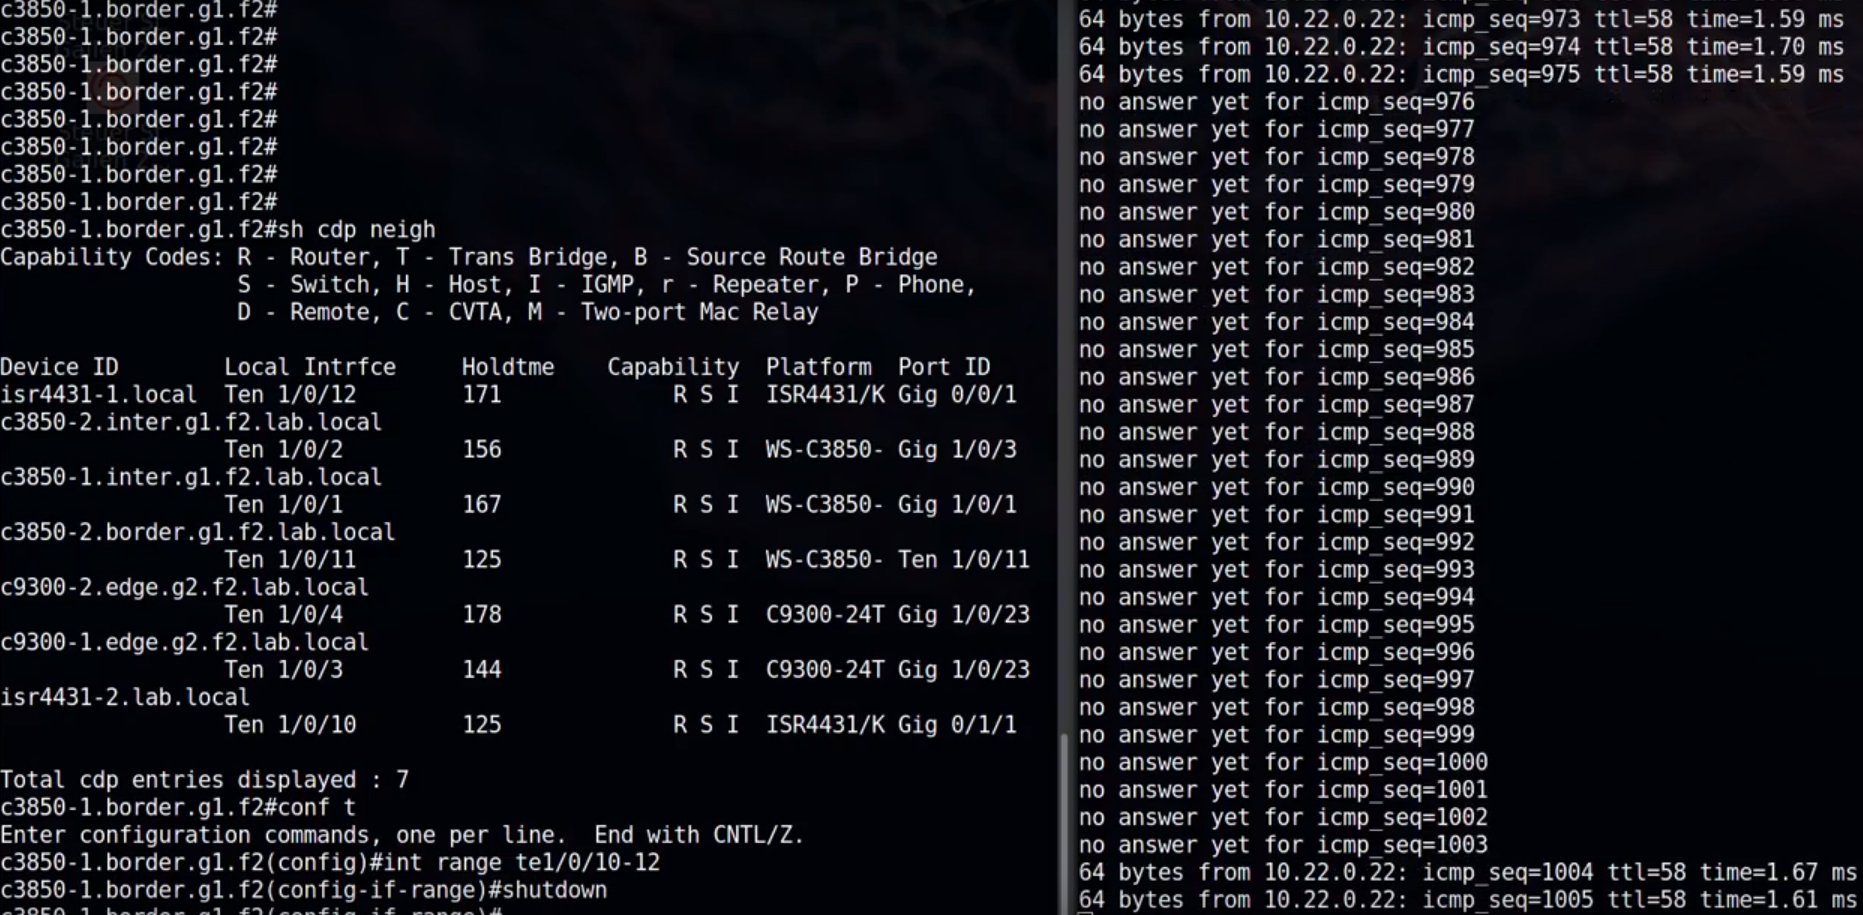
\includegraphics[width=1\linewidth]{img/Absicherung/border-ausfall-test}
	\caption{Border Ausfall Test}
	\label{fig:Border Ausfall Test}
\end{figure}

\subsection{Fusion Router}
Die Fusion Router stellen die Verbindungen zwischen den einzelnen Fabrics, dem Internet, sowie die Verbindung zum Legacy Netzwerk in dem sich beispielsweise das DNAC und der ISE befinden.Es werden mehrere Fusion Router verwendet, um die nötige Ausfallsicherheit zu gewährleisten. Die Fusion Router und Border Nodes sind im Optimalfall in einem Full-Mesh verkabelt. Für das Routing zwischen den Fusion Routern, sowie den Border Nodes kommt BGP zum Einsatz.

Die Topologie wurde analog anhand der nachfolgenden Validation Topologie von Cisco aufgebaut.
\begin{figure}[H]
	\centering
	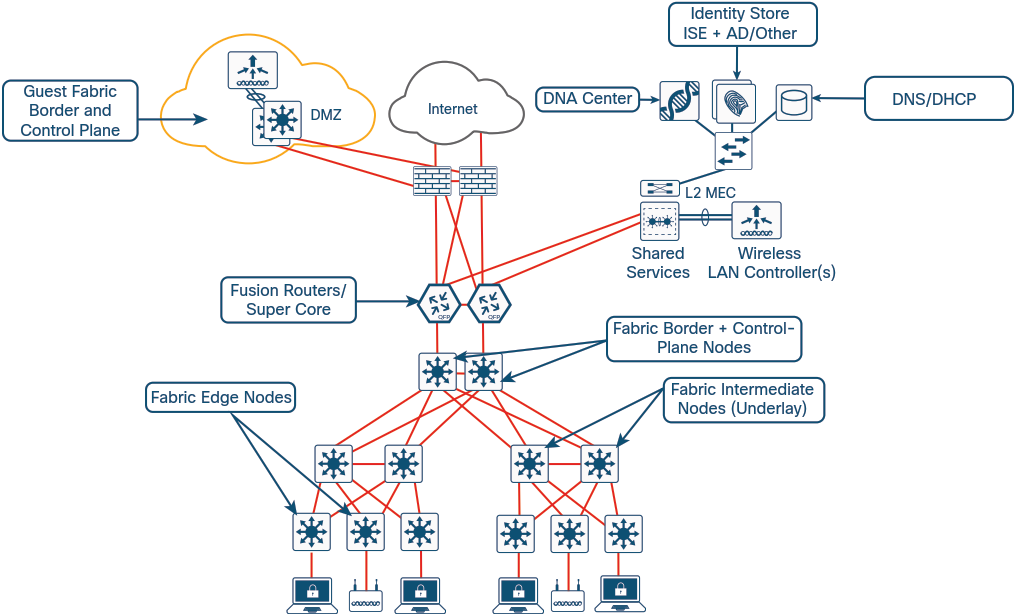
\includegraphics[width=1\linewidth]{img/Absicherung/FusionRouter-ValidationTopology}
	\caption{Fusion Router Validation Topology \cite{sda-deploymentguide-oct2018} }
	\label{fig:Fusion Router Validation Topology}
\end{figure}

\subsubsection{Absicherung Fusion Router}
Wie auch beim Border Node ist darauf zu achten, dass pro Site mindestens zwei Fusion Router vorhanden sind. Dies ist insbesondere dann wichtig, wenn die Kommunkation zwischen den verschiedenen VNs gewährleistet sein muss. Um auch gegen einen Ausfall einer Verbindung abgesichert zu sein, müssen Verbindungen zu den Border Nodes, aber auch zu externen Netzwerken redundant ausgelegt sein.

\subsubsection{Test Ausfall Fusion Router}

Ein Ausfall eines Fusion Routers führt wie ein Ausfall eines Border Nodes zu einem teilweisen Verbindungsunterbruch im Bereich von wenigen Sekunden. In dieser Zeit kann BGP auf die neue Topologie reagieren und alle Pfade wiederherstellen.

\subsection{Absicherung Infoblox}

Infoblox stellt kritische Dienste wie DHCP, DNS und NTP für Netzwerkgeräte und Clients zur Verfügung. Aus diesem Grund muss die Verfügbarkeit dieser Services immer gewährleistet sein.

\subsubsection{HA-Pairs}
Zwei Infoblox Instanzen können in einem High-Availability Pair betrieben werden. Damit sind alle Services redundant und ein Ausfall einer einzelnen Instanz hat keinen Einfluss auf den Betrieb. 

\subsubsection{Grid}
Infoblox kann in einem Grid betrieben werden. Dies bedeutet, es gibt einen Grid Master und mehrere Grid Member. Alle Konfigurationen werden auf dem Grid Master definiert. Des Weiteren kann definiert werden, welche Member für spezifische Services zuständig sind. Somit kann sichergestellt werden, dass an Aussenstandorten nur die Services betrieben werden, die dort auch nötig sind. Um die Ausfallsicherheit weiter zu erhöhen, können Grid Master und Member zusätzlich als High-Availability Pair betrieben werden.

\paragraph{Grid Member hinzufügen}

Ein neuer Grid Member kann im UI von Infoblox unter \textit{Grid $\rightarrow$ Grid Manager $\rightarrow$ Members} hinzugefügt werden.

\begin{figure}[H]
	\centering
	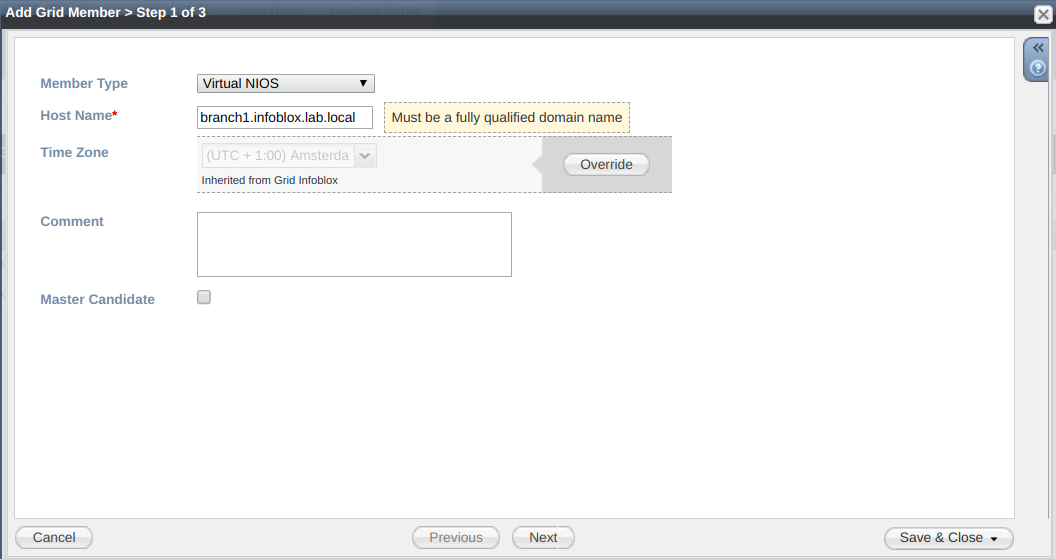
\includegraphics[width=1\linewidth]{img/Absicherung/Infoblox_Add_Grid_Member.png}
	\caption{Infoblox - Add Grid Member}
	\label{fig:Infoblox - Add Grid Member}
\end{figure}

\paragraph{Member Assignment}

Sobald die Grid Member hinzugefügt wurden, kann definiert werden, für welche Services diese zuständig sind. Dies kann sehr granular definiert werden. Beispielsweise kann für eine einzelne DNS Zone oder einen einzelnen DHCP Pool definiert werden, welche Member zuständig sind.

\begin{figure}[H]
	\centering
	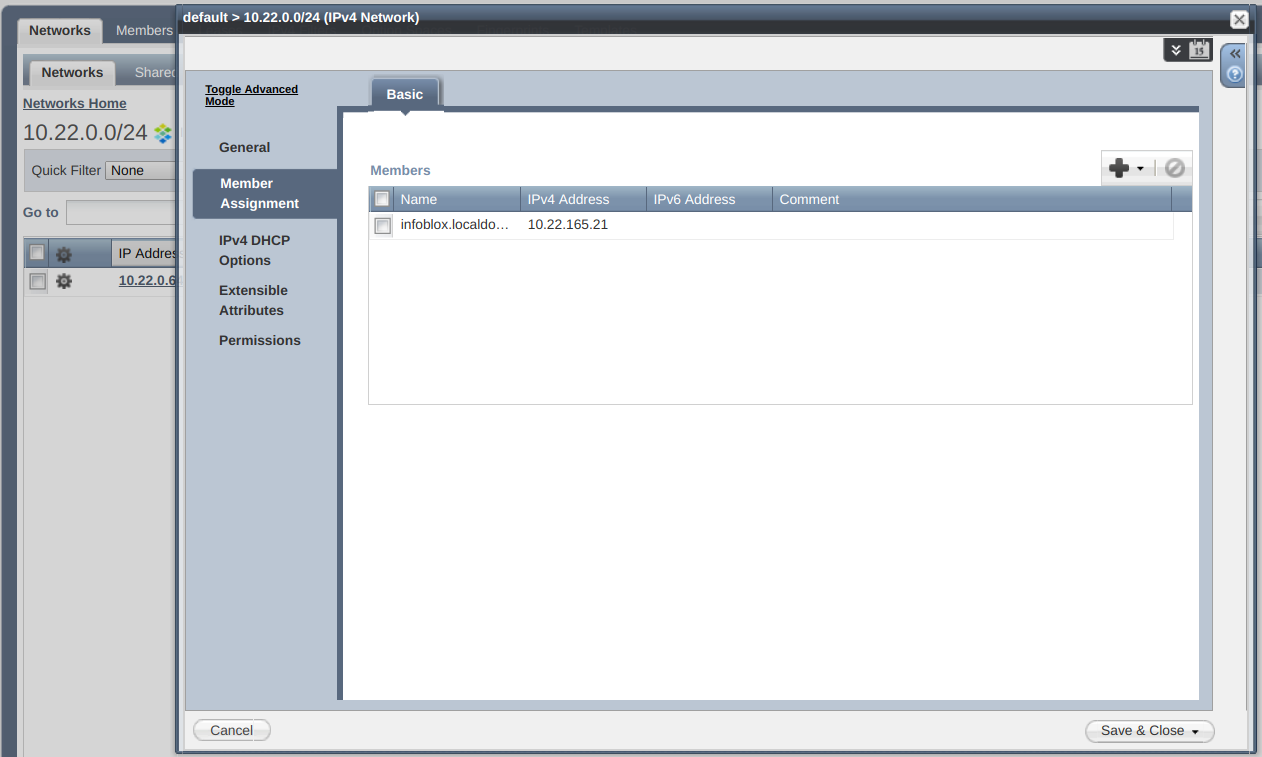
\includegraphics[width=1\linewidth]{img/Absicherung/Infoblox_Member_Assignment.png}
	\caption{Infoblox - Member Assignment}
	\label{fig:Infoblox - Member Assignment}
\end{figure}

\paragraph{Infoblox Services}

Damit alle Services, die Infoblox zur Verfügung stellt, stets an allen Standorten verfügbar sind, müssen die Clients primär die lokale Instanz von Infoblox verwenden. Diese kann auf einem ENCS 5400 oder einer anderen Virtualisierungsplattform betrieben werden.

\subparagraph{DNS}

Werden an den Aussenstandorten Infoblox Instanzen verwendet, kann auf dem Grid Master definiert welche Instanzen was für Zonen zur Verfügung stellen. Somit können Clients an Aussenstellen alle nötigen Zonen auflösen.
Im DNA Center müssen unter \textit{Design $\rightarrow$ Network Settings} jeweils die DNS Server vom entsprechenden Standort konfiguriert werden. Der Server am Hauptstandort kann als zweiter Server eingetragen werden.
Auch die Clients müssen die korrekten Server verwenden. Dies hat den Vorteil, dass die Antwortzeiten möglichst kurz sind und DNS auch im Falle eines Unterbruchs zum Hauptstandort zur Verfügung steht. Sofern diese ihre IP Adresse mittels DHCP beziehen, kann der DNS Server entsprechend gesetzt werden. Ansonsten muss diese Konfiguration manuell vorgenommen werden.

\begin{figure}[H]
	\centering
	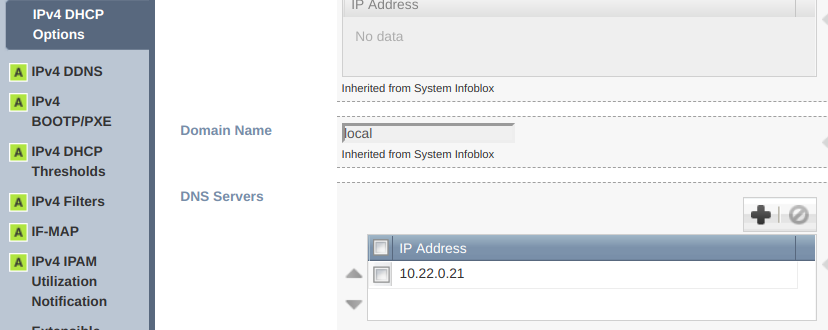
\includegraphics[width=1\linewidth]{img/Absicherung/Infoblox_DHCP_DNS_Server.png}
	\caption{Infoblox - DNS Server}
	\label{fig:Infoblox - DNS Server}
\end{figure}

\subparagraph{DHCP}

Wie auch bei DNS ist es wichtig, dass an Aussenstandorten stets der lokale DHCP Server verwendet wird. Dies kann im DNA Center unter \textit{Design $\rightarrow$ Network Settings} für jeden Standort konfiguriert werden. 

\begin{figure}[H]
	\centering
	
\includegraphics[width=0.8\linewidth]{img/Absicherung/DNA_Center_DHCP-Server.png}
	\caption{DNA Center - DHCP Server }
	\label{fig:DNA Center - DHCP Server}
\end{figure}

Ist an einem Standort eine Hochverfügbarkeit des DHCP Services nötig, wird empfohlen, an diesem Standort ein High-Availability Pair zu betreiben.

\subparagraph{NTP}

Für NTP ist es besonders wichtig, dass dieser Dienst stets verfügbar und möglichst nahe beim Client ist. Wird der NTP Dienst also an jedem Standort mit Infoblox betrieben kann die nötige Verfügbarkeit gewährleistet werden und die Zeitabweichungen sind minimal.
Auch hier, kann der NTP Server für die Netzwerkgeräte im DNA Center unter \textit{Design $\rightarrow$ Network Settings} individuell für jeden Standort konfiguriert werden. Für die Clients empfiehlt sich die DHCP Option 42. Mit dieser können den Clients die korrekten NTP Server mitgeteilt werden.

\begin{figure}[H]
	\centering
	
\includegraphics[width=0.8\linewidth]{img/Absicherung/Infoblox_NTP_Server.png}
	\caption{Infoblox - NTP Server }
	\label{fig:Infoblox - NTP Server}
\end{figure}

Die NTP Server an den Aussenstandorten verwenden als primäre Quelle die NTP Server am Hauptstandort. Um einen Ausfall der Verbindung zu diesem abzusichern, sollte aber auch mindestens ein externen NTP Server konfiguriert werden.

\subsection{Third Party Software}

Alternativ zu Infoblox Instanzen an allen Standorten können die Services auch mittels Third-Party Software angeboten werden.

\subsubsection{DHCP}

\paragraph{Aussenstellen}
Da sich Infoblox nicht in Kombination mit 3rd Party Software in einem Cluster oder einer Failoverlösung betreiben lässt, müssen an Aussenstandorten eigenständige DHCP Server betrieben werden, um deren Autonomie sicherzustellen. Da Infoblox den isc-dhcp-server für seine DHCP Services verwendet, sollte auch dieser an Aussenstandorten eingesetzt werden. Dieser kann auf einem Linux Server, optimalerweise virtualisiert auf dem ENCS 5400, betrieben werden.
Für wichtige Aussenstandorte kann der isc-dhcp-server in einem Master-Slave Cluster betrieben werden. Somit ist an diesen Standorten ebenfalls eine Ausfallsicherheit gewährleistet.

\subsubsection{DNS}

\paragraph{Read Only DNS Server an Aussenstandorten}
	
Damit Aussenstellen nicht auf DNS Server des Hauptstandortes angewiesen sind, kann in jedem Standort ein Read-Only Server betrieben werden. Somit funktioniert die Namensauflösung auch im Falle eines Kommunikationsverlusts zum Hauptstandort. 

\begin{figure}[H]
	\centering
	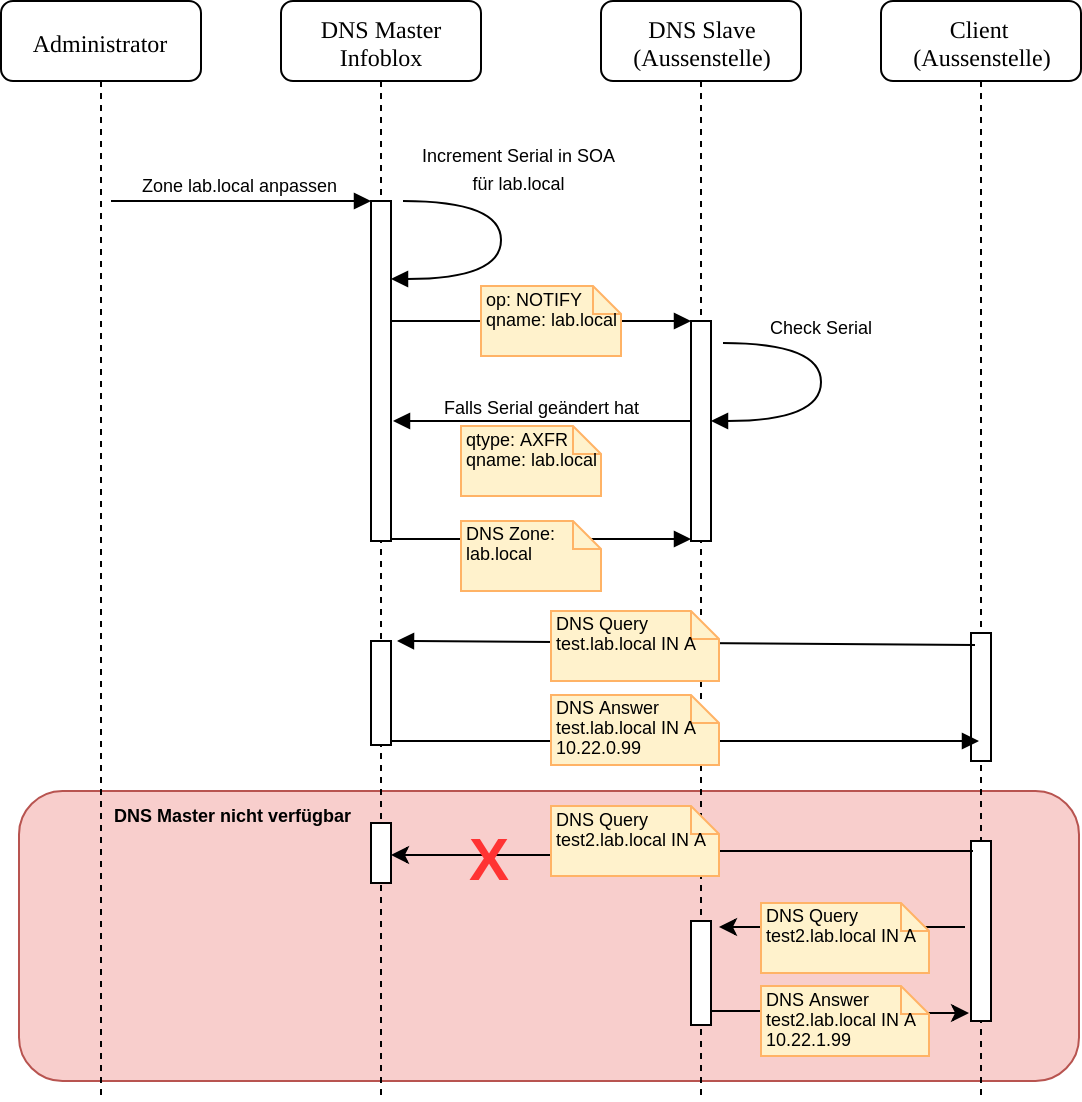
\includegraphics[width=0.8\linewidth]{img/Absicherung/DNS_Sequenzdiagram.png}
	\caption{DNS Sequenzdiagramm}
	\label{fig:DNS Sequenzdiagramm}
\end{figure}

\paragraph{Infoblox}

Damit die Read-Only Server stets über die aktuellsten DNS Zonen verfügen, müssen die Informationen von Infoblox auf diese repliziert werden. In diesem Fall wird dafür der Zone Transfer verwendet. Dazu muss dies in Infoblox für alle Slave Server erlaubt werden. 

Dies wird in Infoblox via \textit{Grid $\rightarrow$ DNS $\rightarrow$ Infoblox Instanz $\rightarrow$ Edit $\rightarrow$ Zone Transfers} ausgeführt.

\begin{figure}[H]
	\centering
	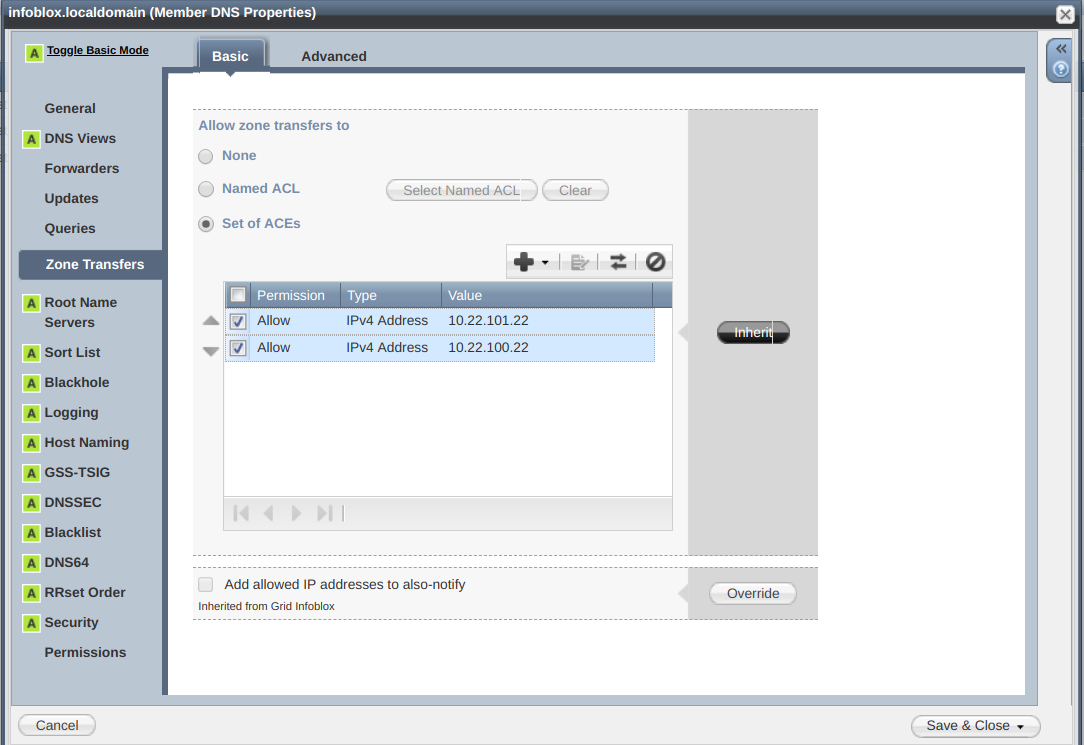
\includegraphics[width=0.8\linewidth]{img/Absicherung/Infoblox_Zone_Transfer.png}
	\caption{Infoblox Zone Transfer}
	\label{fig:Infoblox Zone Transfer}
\end{figure}

\paragraph{DNS Slaves}

Auf den Slaves an den jeweiligen Aussenstandorten müssen die Zonen als Slave Zonen konfiguriert sein und Infoblox muss als Master konfiguriert werden. Dadurch können die Zonen vom Master auf den Slave transferiert werden. Der Slave aktualisiert alle Slave Zonen in regelmässigen Abständen. Dieser Intervall wird in der Zone im SOA Record mit dem "Refresh" Parameter definiert.
Zusätzlich kann auf dem Master konfiguriert werden, dass alle Slaves mittels "Notify" informiert werden, sobald sich eine Zone ändert, worauf der Slave die aktuellsten Informationen für diese Zone abruft. Somit ist sichergestellt, dass alle Server an Aussenstandorten stets über eine aktuelle Konfiguration verfügen.
Auf Grund der grossen Verbreitung sollte bind verwendet werden. Auch Infoblox setzt dieses Produkt ein. Dieses kann, wie auch der isc-dhcp-server auf einem Linux Server betrieben werden.

\subsection{Scheduled Software Updates}
Alle Netzwerk Devices die über das DNA Center verwaltet werden, erhalten ihre aktuellsten Software Images auch von diesem. Die Images haben teils sehr unterschiedliche Grössen (von 200 MB bis zu 1 GB), weshalb es wichtig ist, dass sich diese schon vor einem Upgrade auf den Geräten befinden. 


\subsubsection{Provision Software Images}
Bevor ein Software Image auf ein Gerät übertragen wird, überprüft das DNA Center auf den einzelnen Geräten, ob dieses auch bereit für ein Update ist. Dazu gehören zum Beispiel das Überprüfen des Geräteverwaltungsstatus, Überprüfung der SCP- und HTTPS-Dateiübertragung, Festplattenspeicher usw. Wenn eine Vorprüfung fehlschlägt, kann die Aktualisierung des Software Images nicht durchgeführt werden. \\

Nun kann das Verteilen der Software Images nach folgendem Ablauf gestartet werden:
\begin{enumerate}
	\item Das Verteilen der Software Images kann im DNA Center unter \textit{Provision} konfiguriert werden.
	\item Nun kann das Gerät, welches aktualisiert werden soll, ausgewählt werden. (Wenn der pre-check erfolgreich war, weisst der Link "Outdatet" in der Spalte "OS Image" ein grünes Häckchen auf.)
	\item In der Dropdown-Liste unter \textit{Actions  $\rightarrow$ Update OS Image} wählen
	\begin{enumerate}
		\item Distribute: Mit einem Klick auf \textit{Now} wird das Verteilen des Images sofort gestartet, oder es wird mit einem Klick auf \textit{Later} an einem spezifischen Zeitpunkt ausgeführt. (Wenn sich das Image bereits auf dem ausgewählten Gerät befindet, wird der Distribute-Vorgang übersprungen und das Image kann direkt aktiviert werden.)
		\item Activate: Mit einem Klick auf \textit{Now} wird die Aktivierung sofort gestartet, oder es wird mit einem Klick auf \textit{Later} an einem spezifischen Zeitpunkt ausgeführt. (Dieser Schritt kann übersprungen werden, wenn zum jetzigen Zeitpunkt nur das Image auf das Gerät verteilt werden sollte.)
		\item Confirm: Mit einem Klick auf \textit{Confirm} wird das Update bestätigt.
	\end{enumerate}
	\item Nun kann unter \textit{Upgrade Status} der aktuelle Vorgang des Image Upgrades beobachtet werden.
\end{enumerate}

Sollte das Verteilen des Software Images nicht funktionieren, in dem es Beispielsweise die Übertragung immer wieder abbricht, so kann das Image auch manuell auf das Gerät kopiert werden. So würde dies bei dem vorher beschriebenen Vorgang \textit{Distribute} automatisch erkennt werden, dass sich das Image schon auf dem Gerät befindet.


